\section{Performance}

\subsection{Module testing}

\begin{figure}[hbt] 
\centering 
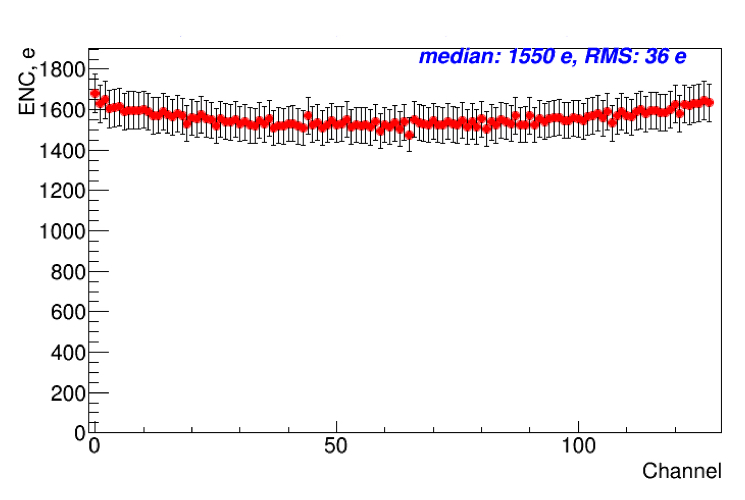
\includegraphics[width=1.0\columnwidth,keepaspectratio]{enc-chip.jpg}
\caption{Typical input noise on a single chip of an SVT module.}
\label{fig:enc-chip}
\end{figure} 

Detailed quality assurance procedures were developed for testing the modules during assembly at Fermilab, reception tests at Jefferson Lab, tracker integration, and commissioning. At each stage the results were compared with previous measurements. Module performance was tested by calibration procedures. No significant correlated noise has been observed between the channels of the same chip, chips of the same module or closely placed modules. The measured average channel noise (see Fig.~\ref{fig:enc-chip}) is comparable with the estimated contributions of different noise sources. The gain dispersion measured on the channels is within the specs of the readout chip (see Fig.~\ref{fig:gain-chip}). To verify operational stability and functionality of the module at low temperature with active cooling, a performance test was conducted at -20 C using a sealed container and a module in a carrier box.

\begin{figure}[hbt] 
\centering 
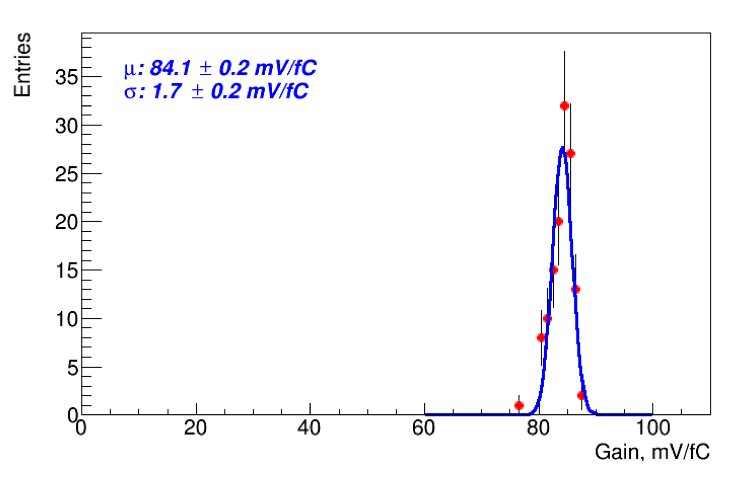
\includegraphics[width=1.0\columnwidth,keepaspectratio]{gain-chip.jpg}
\caption{Distribution of the gain for the channels of one representative FSSR2 ASIC.}
\label{fig:gain-chip}
\end{figure}

\begin{figure}[hbt] 
	\centering 
	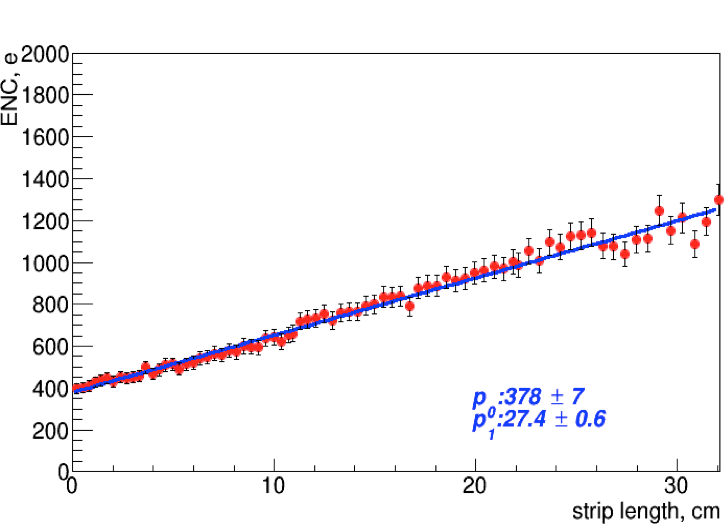
\includegraphics[width=1.0\columnwidth,keepaspectratio]{encstriplength.png}
	\caption{Input noise vs. strip length.}
	\label{fig:encstriplength}
\end{figure}

Longer silicon strips have higher capacitance and thus a higher input noise (see Fig.~\ref{fig:encstriplength}). Noise calibration accounts for the different strip lengths and pitch adapter layouts that affect the input capacitance of the preamplifier. The mean noise values scale linearly with strip length which confirms that the noise is dominated by the strip capacitance and not by coherent noise pickup of the system. The channel noise has a linear dependence on the strip length with the offset p$_{0}$ about 400 electrons (with shaper at 125 ns) corresponding to the ENC for the shortest strips and the slope p$_1$ of 27 electrons, consistent with FSSR2 noise measurements at comparable capacitive load taken on a single-chip test board with discrete capacitors (see Fig.~\ref{fig:fssr2-enc-c}).

\begin{figure}[hbt] 
\centering 
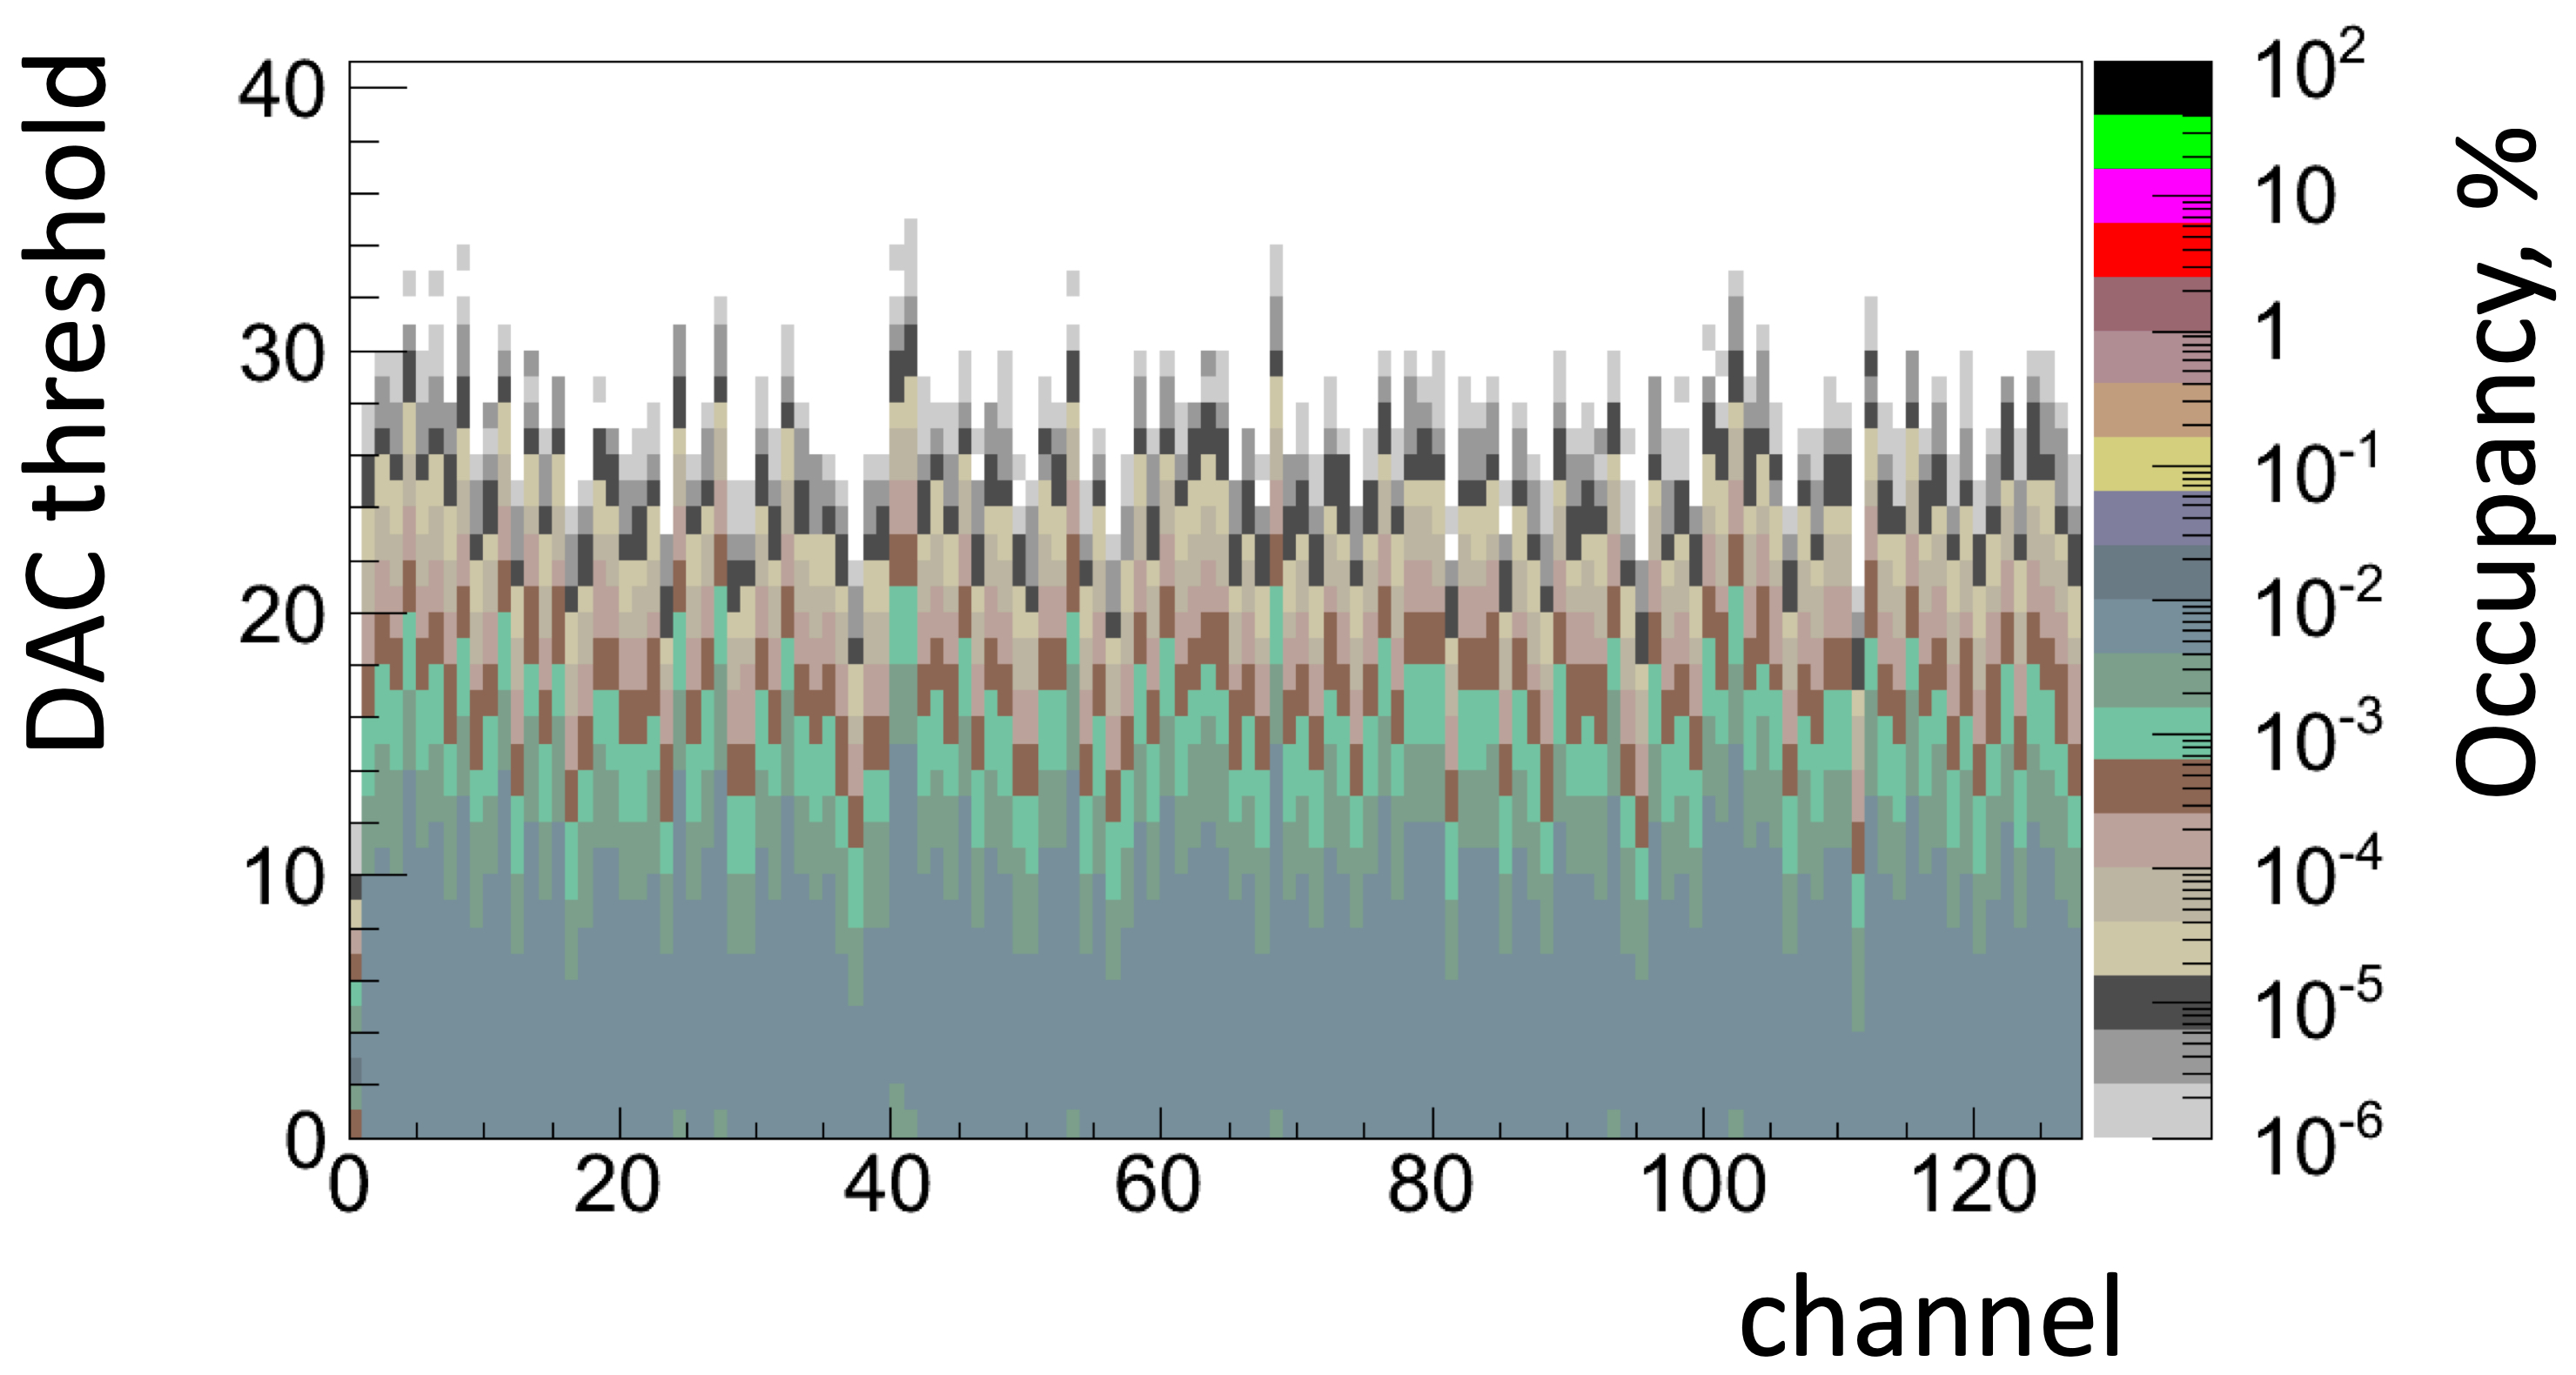
\includegraphics[width=1.0\columnwidth,keepaspectratio]{occ_thr.jpg}
\caption{Channel noise occupancy vs. DAC hit/no-hit threshold (in DAC bins, one DAC bin corresponds to 3.5~mV).}
\label{fig:noiseocc}
\end{figure}

The noise occupancy histogram with no charge injection is used to find the noise value (Fig.~\ref{fig:noiseocc}). It probes the tail of the noise distribution, which can show effects, which are masked by the higher occupancy at low thresholds and provides a cross-check of the noise value obtained from the response curve measurement. A MPV of the signal peak from a MIP corresponds to a 100$^{th}$ DAC bin. The equivalent noise charge of the SVT channels is shown in  Fig.~\ref{fig:enc}. The peak is $\sim$1600 electrons (signal-to-noise ratio 15), the shoulder on the left side is related to the shorter strips. The channel noise allows setting a 3$\sigma$ threshold at the 30~keV level. 

\begin{figure}[hbt] 
	\centering 
	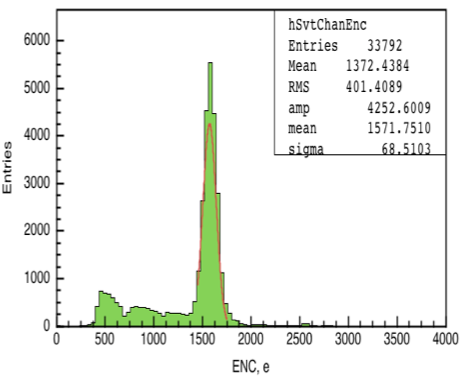
\includegraphics[width=1.0\columnwidth,keepaspectratio]{enc.png}
	\caption{SVT ENC for all channels. The main peak corresponds to the full length strips (33 cm). The shoulder on the left side is related to the shorter strips.}
	\label{fig:enc}
\end{figure}

The detector response and full readout chain calibration was done with $\gamma$ and $\beta$ sources, cosmic muons, electron beam, and proton beam. The output from the 3-bit ADC is not allowing to get a good resolution of the pulse height. To increase the number of bins in the cluster charge distribution, a sliding window method was used, combining the data taken for the same time window in several runs with discriminator thresholds set for the required binning. When using signals from minimum ionizing particles, like cosmic rays or $^{90}$Sr $\beta$ source, the signal distribution is fitted with a Landau-Gauss convolute. The detector response to minimum ionizing particle (MIP) was about 24000 electrons, which is what is expected for the 320 $\mu$m thick sensor. The results of absolute gain calibration with a $\gamma$ source (Am$^{241}$) are shown in Fig.~\ref{fig:signal-gamma}. The signal peak is in good agreement with the expected position (marked with an arrow). 

\begin{figure}[hbt] 
	\centering 
	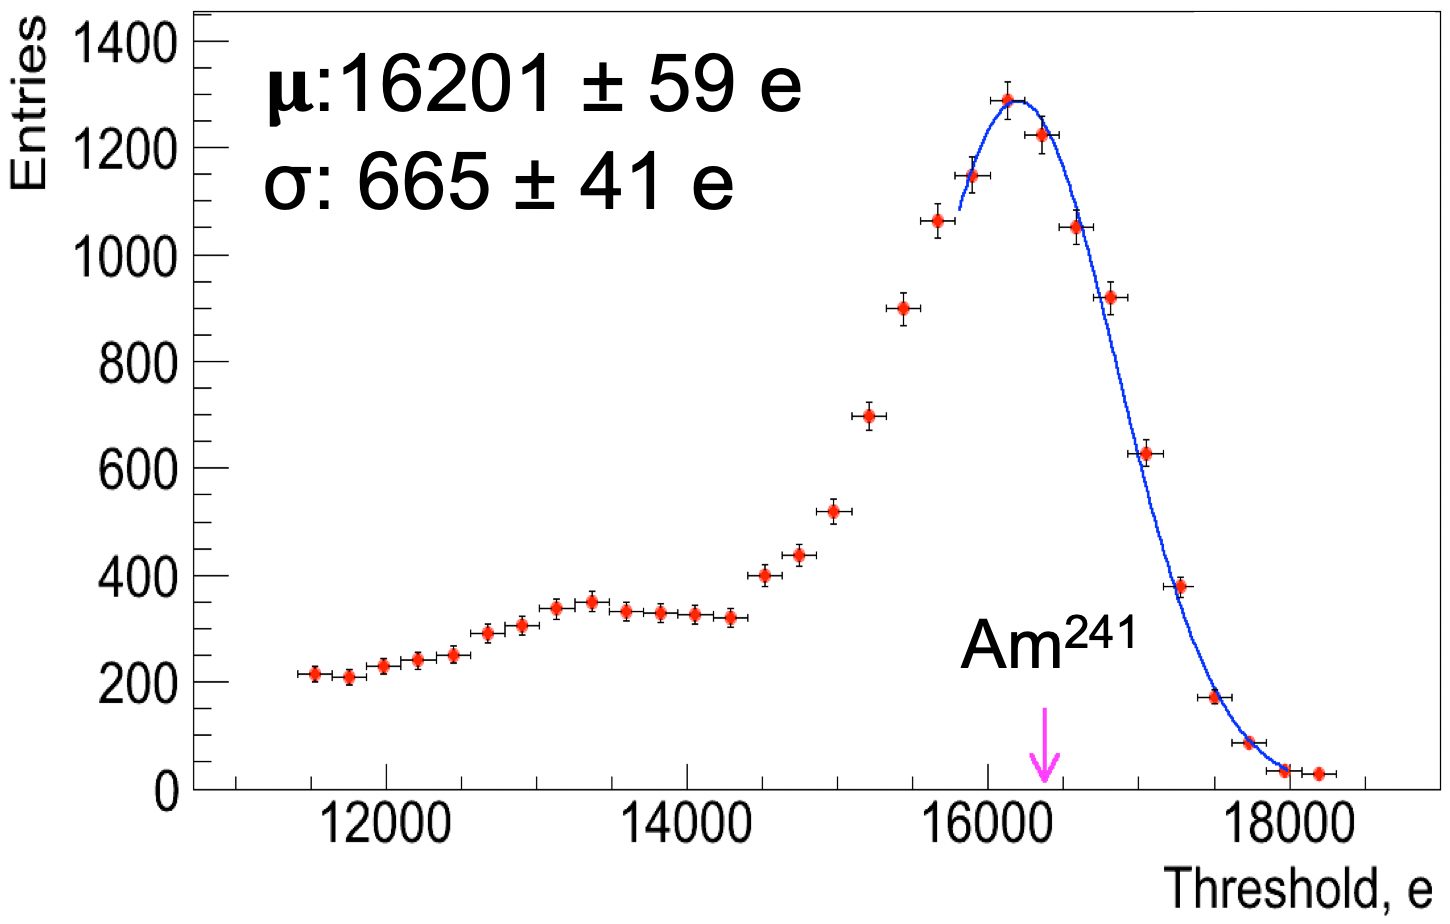
\includegraphics[width=1.0\columnwidth,keepaspectratio]{signal-gamma.jpg}
	\caption{Signal from Am$^{241}$ $\gamma$ source.}
	\label{fig:signal-gamma}
\end{figure}

%
%\begin{wrapfigure}{l}{0.5\columnwidth}
%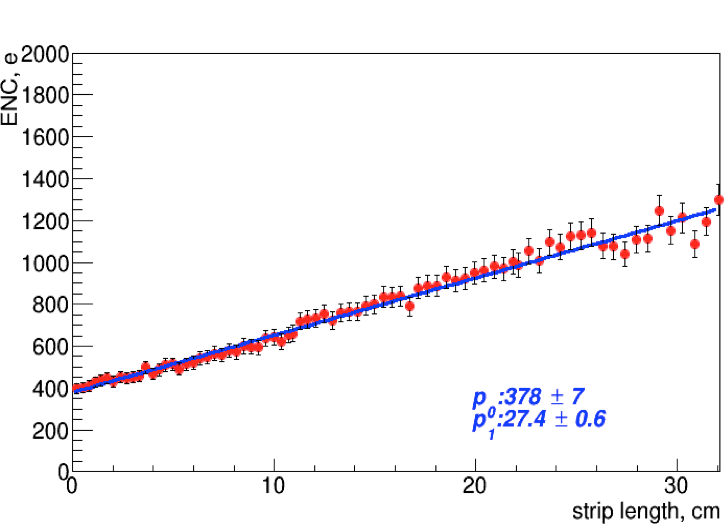
\includegraphics[width=1.0\columnwidth]{encstriplength.png}
%\caption{Input noise vs. strip length.}
%\label{fig:encstriplength}
%\end{wrapfigure}
%Longer silicon strips have higher capacitance and thus a higher expected value for the input noise. 
%(see Fig.~\ref{fig:encstriplength}).
%

%\begin{wrapfigure}{l}{0.5\columnwidth}
%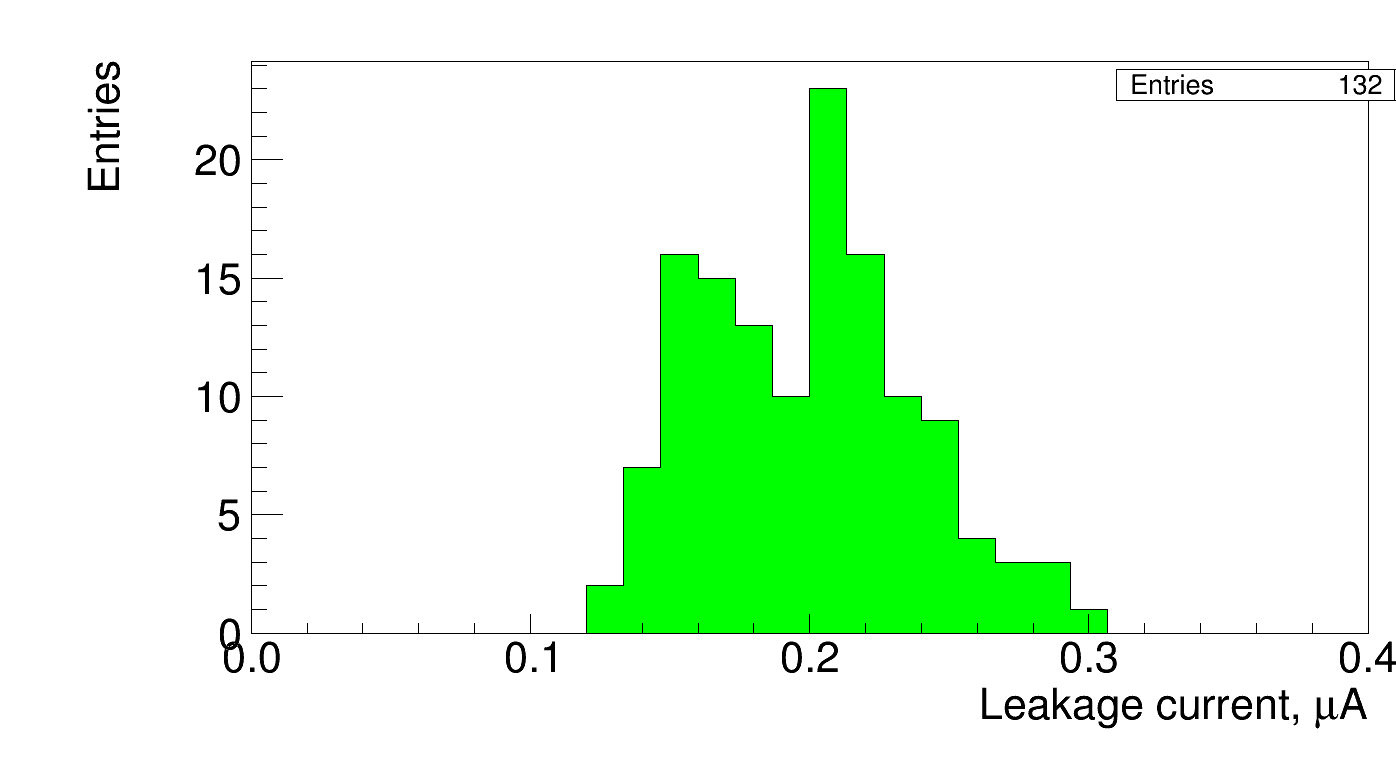
\includegraphics[width=1.0\columnwidth]{currents.png}
%\caption{Leakage currents}
%\label{fig:currents}
%\end{wrapfigure}
%
%\begin{wrapfigure}{l}{0.5\columnwidth}
%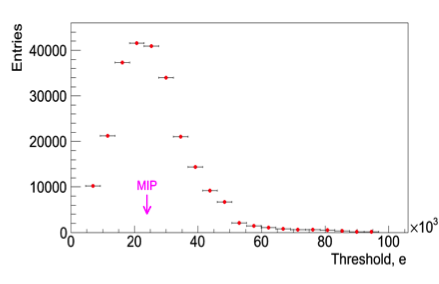
\includegraphics[width=1.0\columnwidth]{signal-muons.png}
%\caption{Signal muons}
%\label{fig:signal-muons}
%\end{wrapfigure}

\subsection{Integration and system checkout}

To verify performance of the integrated detector, data acquisition chain, power services, and cooling system, as well as the detector control and data acquisition software, the final detector system was installed in the clean room and used at all stages of tracker integration and commissioning. The SVT was operated for several months under environmental conditions close to the ones in the experimental hall. Defects known before the integration of the system were reestablished. 99.9$\%$ of channels were operational after the detector integration. 
 
\begin{figure}[hbt] 
\centering 
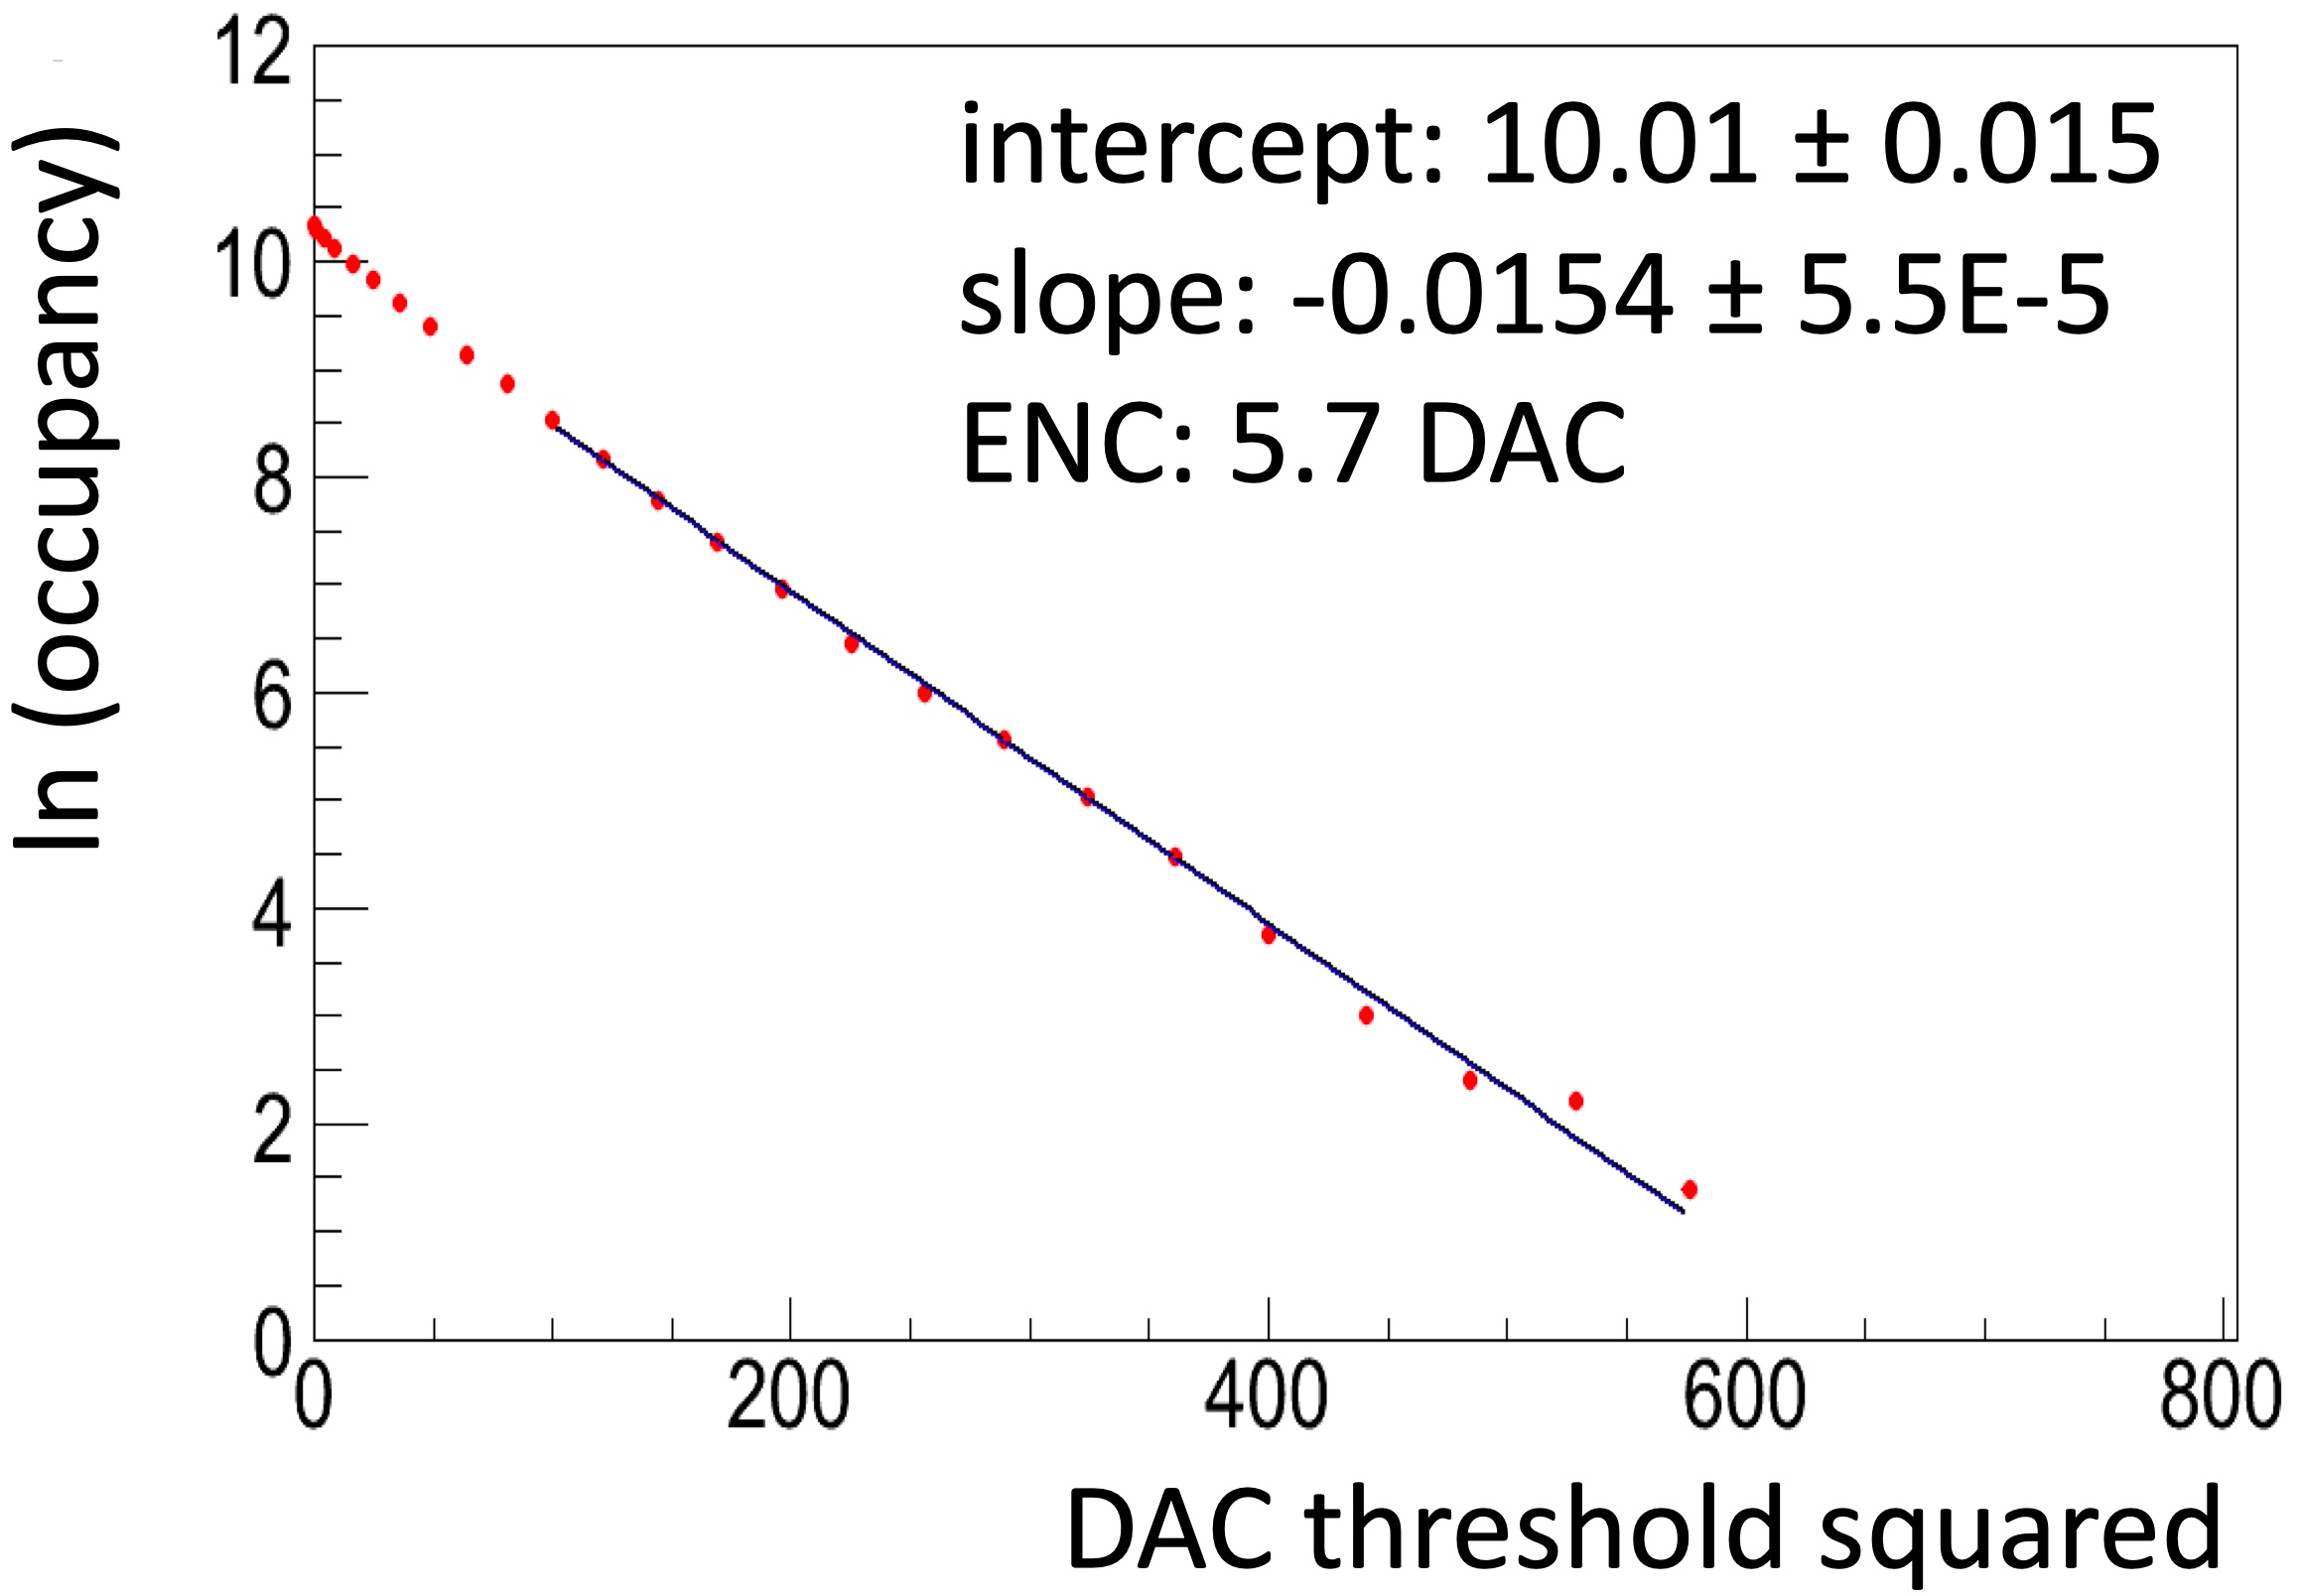
\includegraphics[width=1.0\columnwidth,keepaspectratio]{occupancy-threshold.jpg}
\caption{Log occupancy vs. threshold squared.}
\label{fig:occupancy-threshold}
\end{figure}

The noise behavior was found to be within expectations and well understood. The dependence of the noise on the environmental temperature and humidity is small. The noise performance in the experimental hall was comparable with the results taken in the clean room during integration. Several diagnostic tools were used to measure the common mode noise performance of the detector. Fig.~\ref{fig:occupancy-threshold} shows log occupancy vs. threshold squared plot. Purely Gaussian noise gives a straight line in the plot over much of the useful range. Occupancy refers to the (normalized) total number of hits in all channels in a run. The power of this plot is to show non-Gaussian noise contributions as deviations from this linear fall-off. The hit map is plotted in the plane spanned by channel number and event number. It is an important diagnostic tool to test for presence of the correlated noise and understanding the data quality, such as dead/noisy channels, channel occupancy, uniformity across the channels and events in a run, coherent effects on the channels in individual events.

\begin{figure}[hbt] 
\centering 
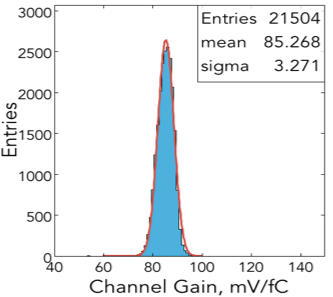
\includegraphics[width=1.0\columnwidth,keepaspectratio]{svt_gain.png}
\caption{Distribution of gain for the SVT channels.}
\label{fig:svt_gain}
\end{figure}

No significant correlated noise has been observed between the channels of the same chip, between the chips of the same module, or between the closely placed modules. The front-end electronics performed reliably, and no chip failures were observed. The distribution of gain was uniform and stable for all channels (see Fig.~\ref{fig:svt_gain}). 
 
\begin{figure}[hbt] 
\centering 
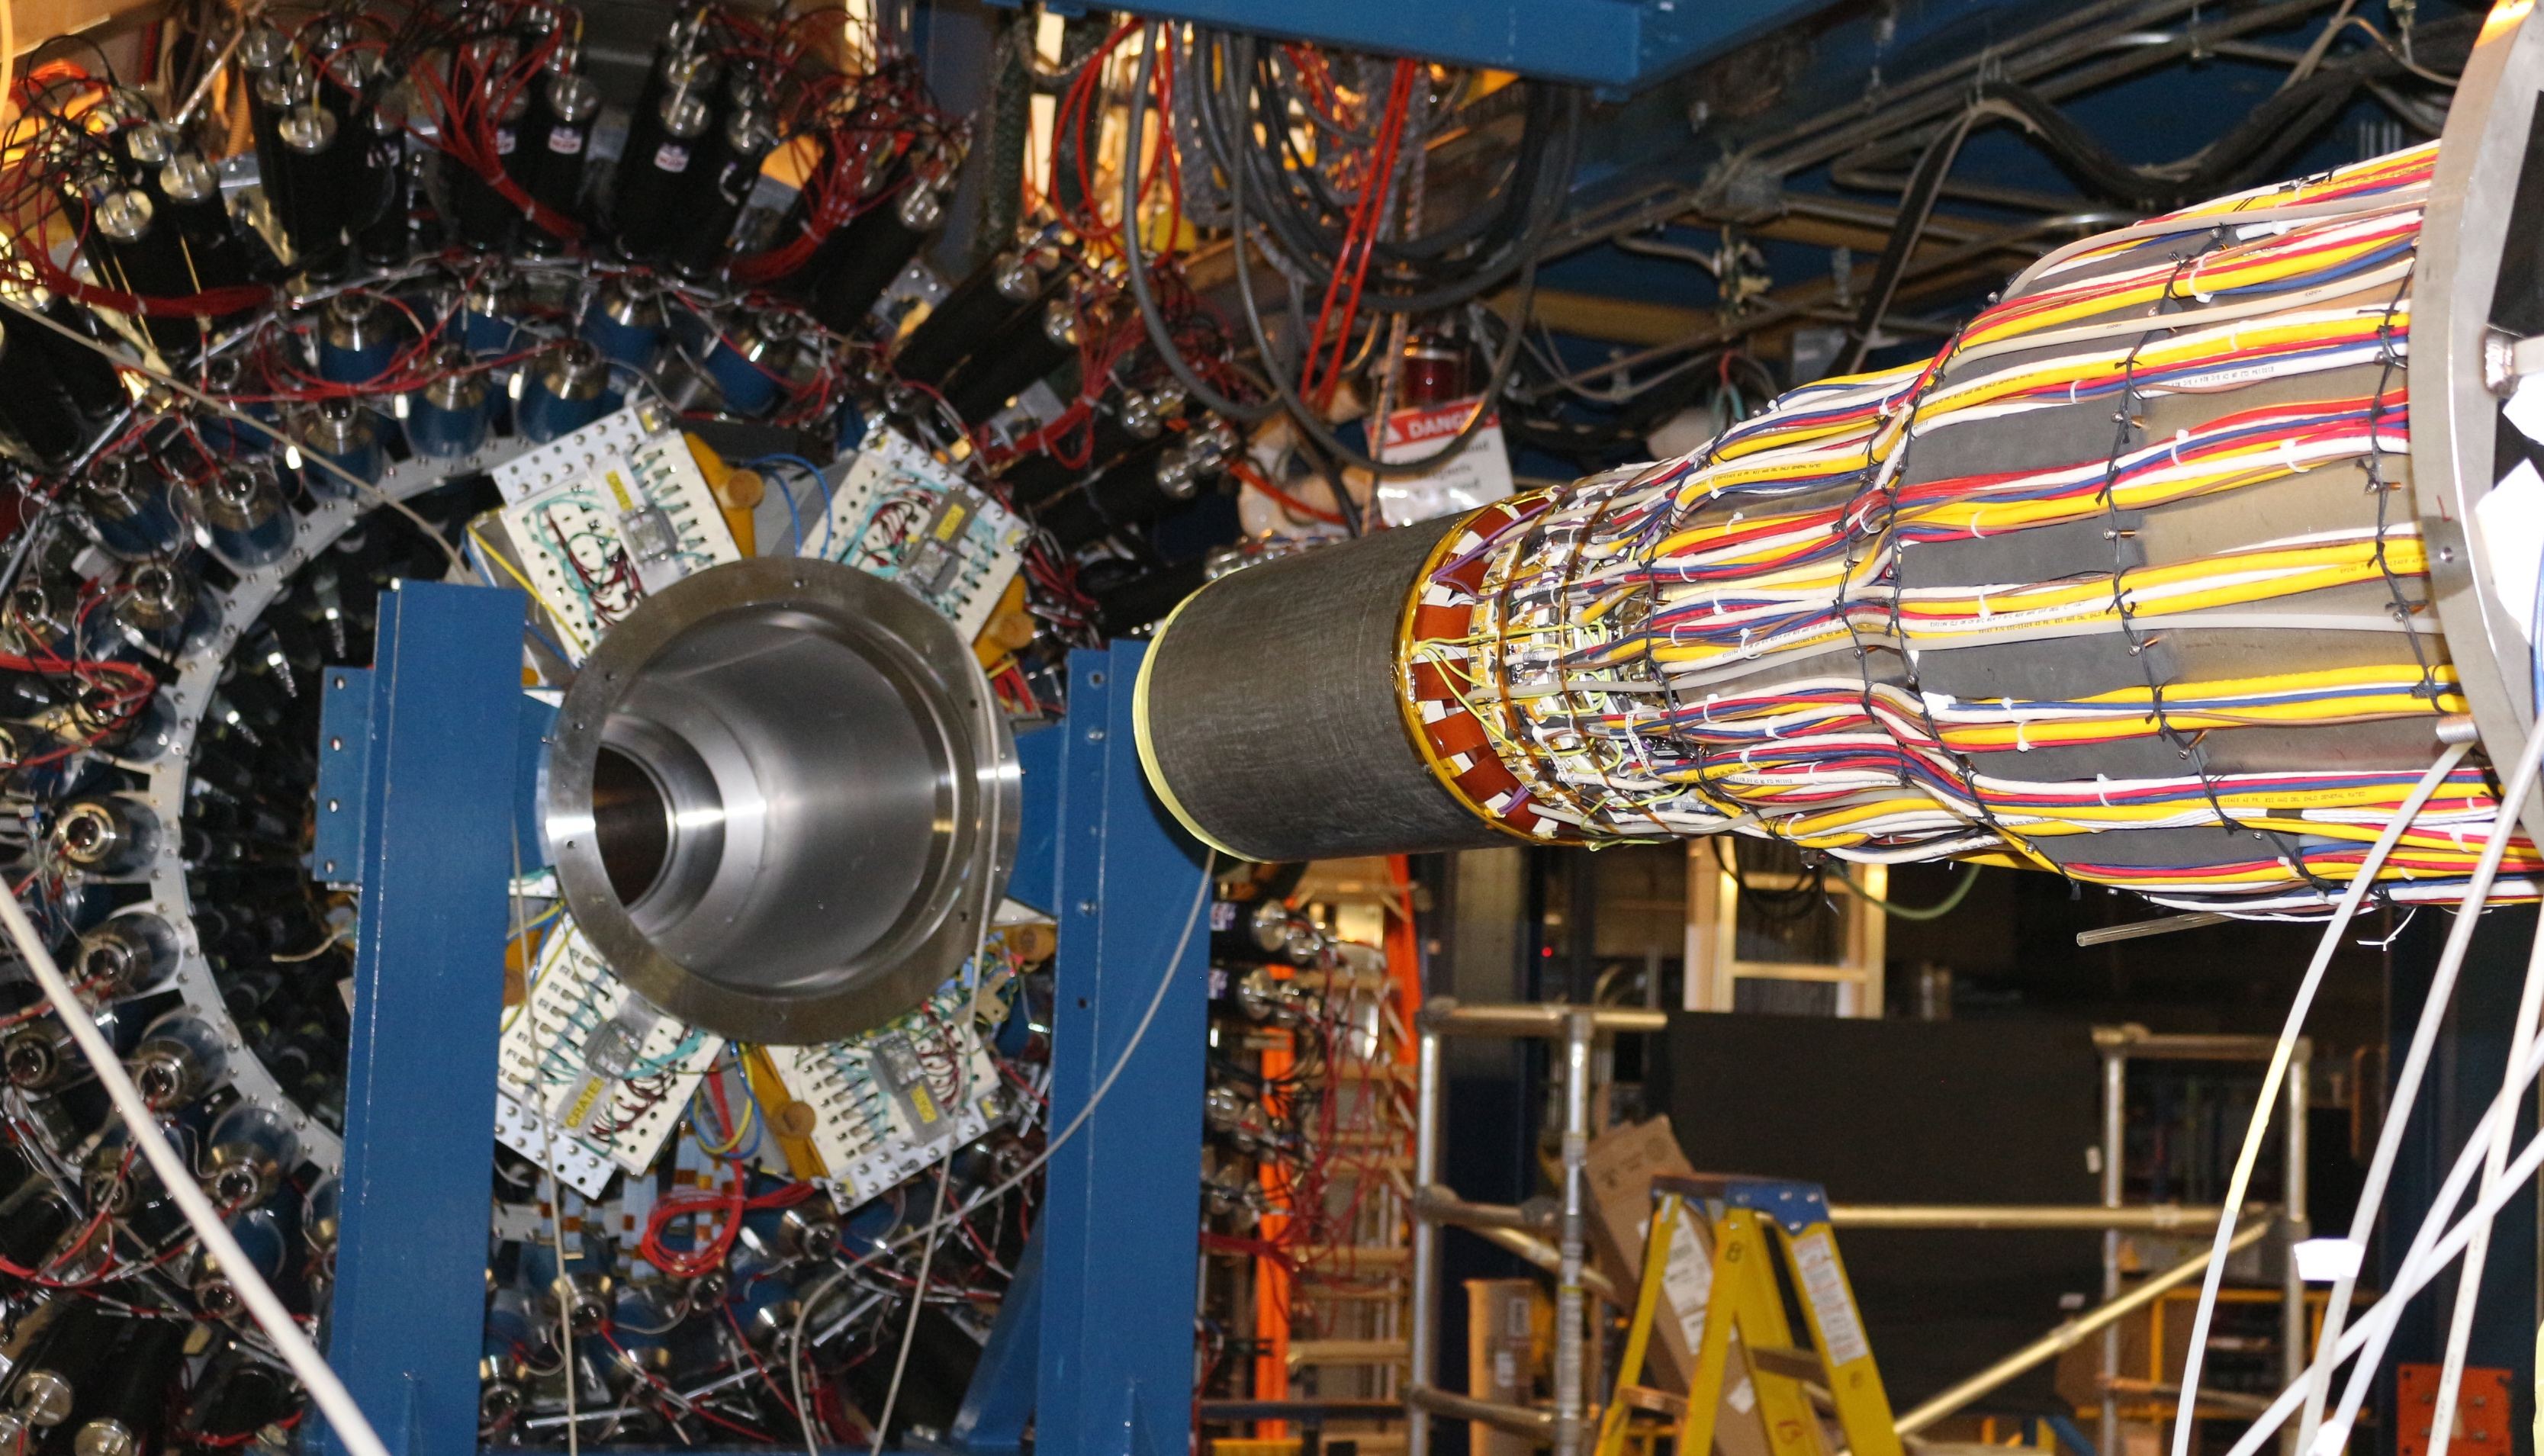
\includegraphics[width=1.0\columnwidth,keepaspectratio]{svt-hall.jpg}
\caption{SVT detector installed in the experimental hall before being integrated with the CLAS12 detector.}
\label{fig:svt-hall}
\end{figure}

In the hall the SVT was dismounted from the integration cart, craned to the space frame level in horizontal position using the mounting brackets on the support tube and the counter weight system to balance the weight of the cables which remained connected to the modules and coiled around the support tube during this operation. The support tube was attached to the central tracker service cart with alignment system for final adjustment of the SVT along the beam line. The cart hosts the crates for the power supplies, back-end electronics, slow controls, and the dry air distribution system. The service cart is placed on the wheels and can be moved along the beam line on the rails, providing access to the detector during maintenance. The power, network, gas, and cooling lines are long enough to allow the cart to be moved up to 5 m upstream. Fig.~\ref{fig:svt-hall} shows the SVT detector after installation in the experimental hall. All modules were found to be fully functional after transportation from the assembly site and installation on the beam line. 

\begin{figure}[hbt] 
\centering 
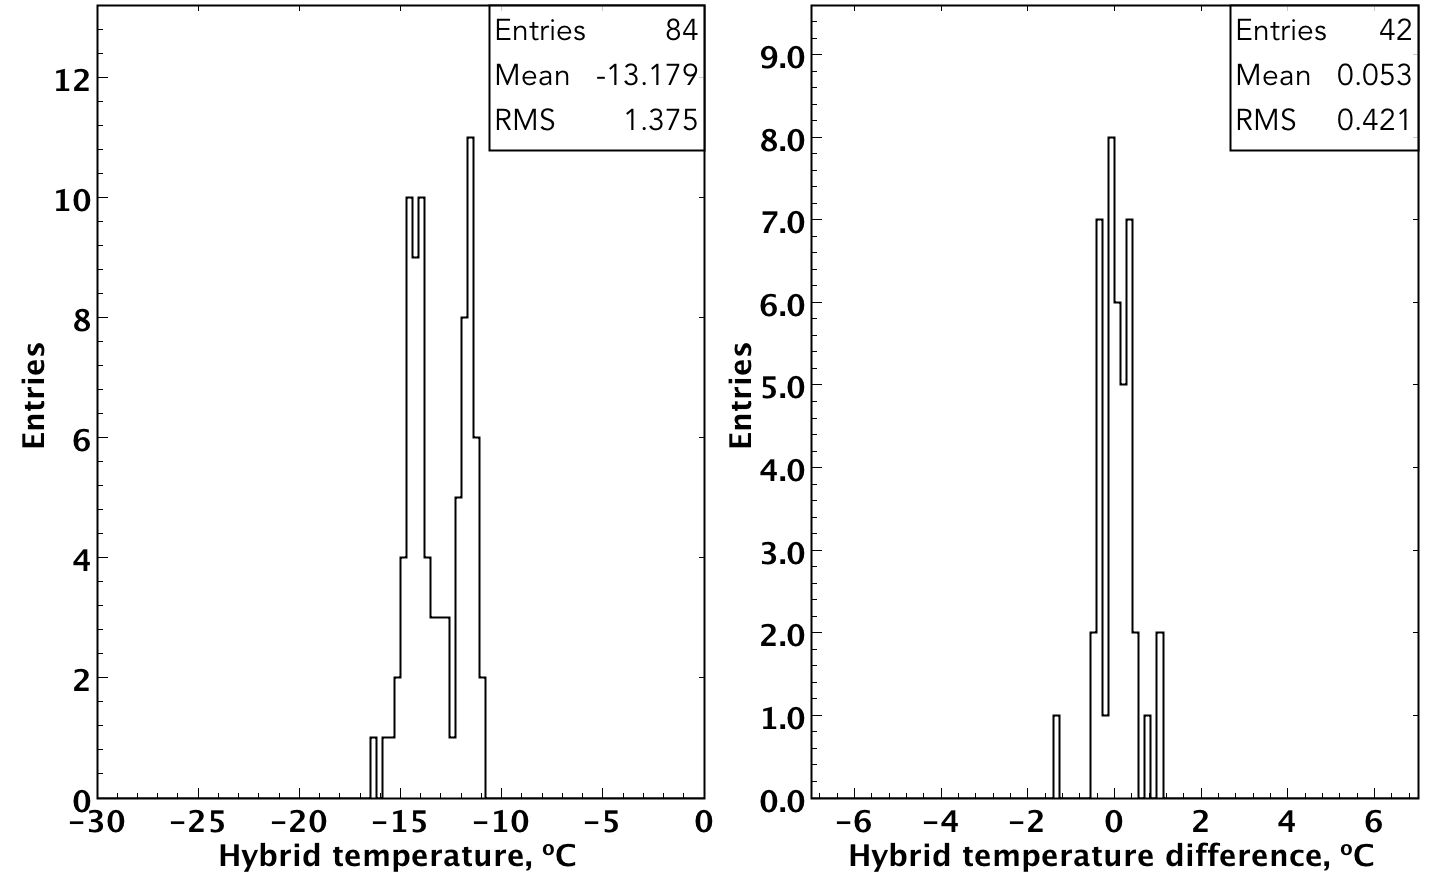
\includegraphics[width=1.0\columnwidth,keepaspectratio]{hybrid-temps.png}
\caption{Hybrid temperatures (left) and the difference in temperature between the two sides of the module with coolant at -26 $^\circ$C (right).}
\label{fig:hybrid-temps}
\end{figure}

Temperature variation of the SVT modules measured by sensors mounted on the hybrids with coolant at -26 $^\circ$C is shown in Fig.~\ref{fig:hybrid-temps} (left). In these operating conditions the module temperatures were uniformly distributed within the region, with lower temperatures close to the cooling lines. Region 3 temperatures were slightly higher than in the inner regions. The temperature difference between the two sides of a module is within 1$^\circ$C as shown in Fig.~\ref{fig:hybrid-temps} (right). Sensor leakage currents remained at the same low levels after installation (see Fig.~\ref{fig:currents}). Thermal cycling of the modules verified the robustness of the bond wires.

\begin{figure}[hbt] 
\centering 
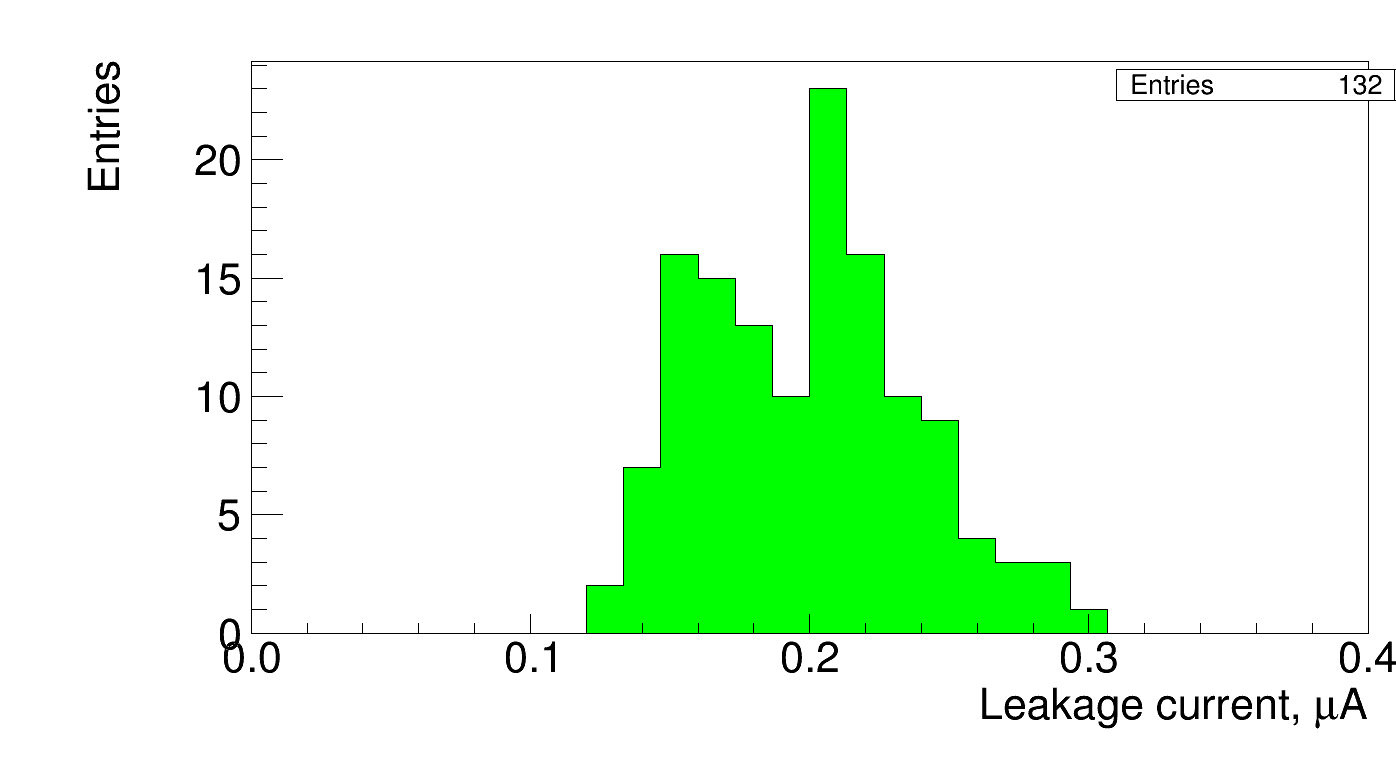
\includegraphics[width=1.0\columnwidth,keepaspectratio]{currents.png}
\caption{Sensor leakage currents after detector integration.}
\label{fig:currents}
\end{figure}

\subsection{Commissioning with cosmic rays}

Cosmic ray tests of the SVT have been used to test track reconstruction routines for the SVT, qualify the geometrical precision of detector assembly by track based alignment methods, establish correct readout, good noise performance, full response for the entire detector, measure the inter-strip couplings, study the time evolution of the detector response. 
Once the reception tests of the first assembled modules were complete, a cosmic test stand was assembled (Fig.~\ref{fig:cosmic-stand}) to verify the expected performance of the detector. Four SVT modules were stacked vertically between the two trigger paddles. Evaluation of the signal to noise ratio and capacitive coupling confirmed the estimates and validated the full readout chain calibration data.

\begin{figure}[hbt] 
\centering 
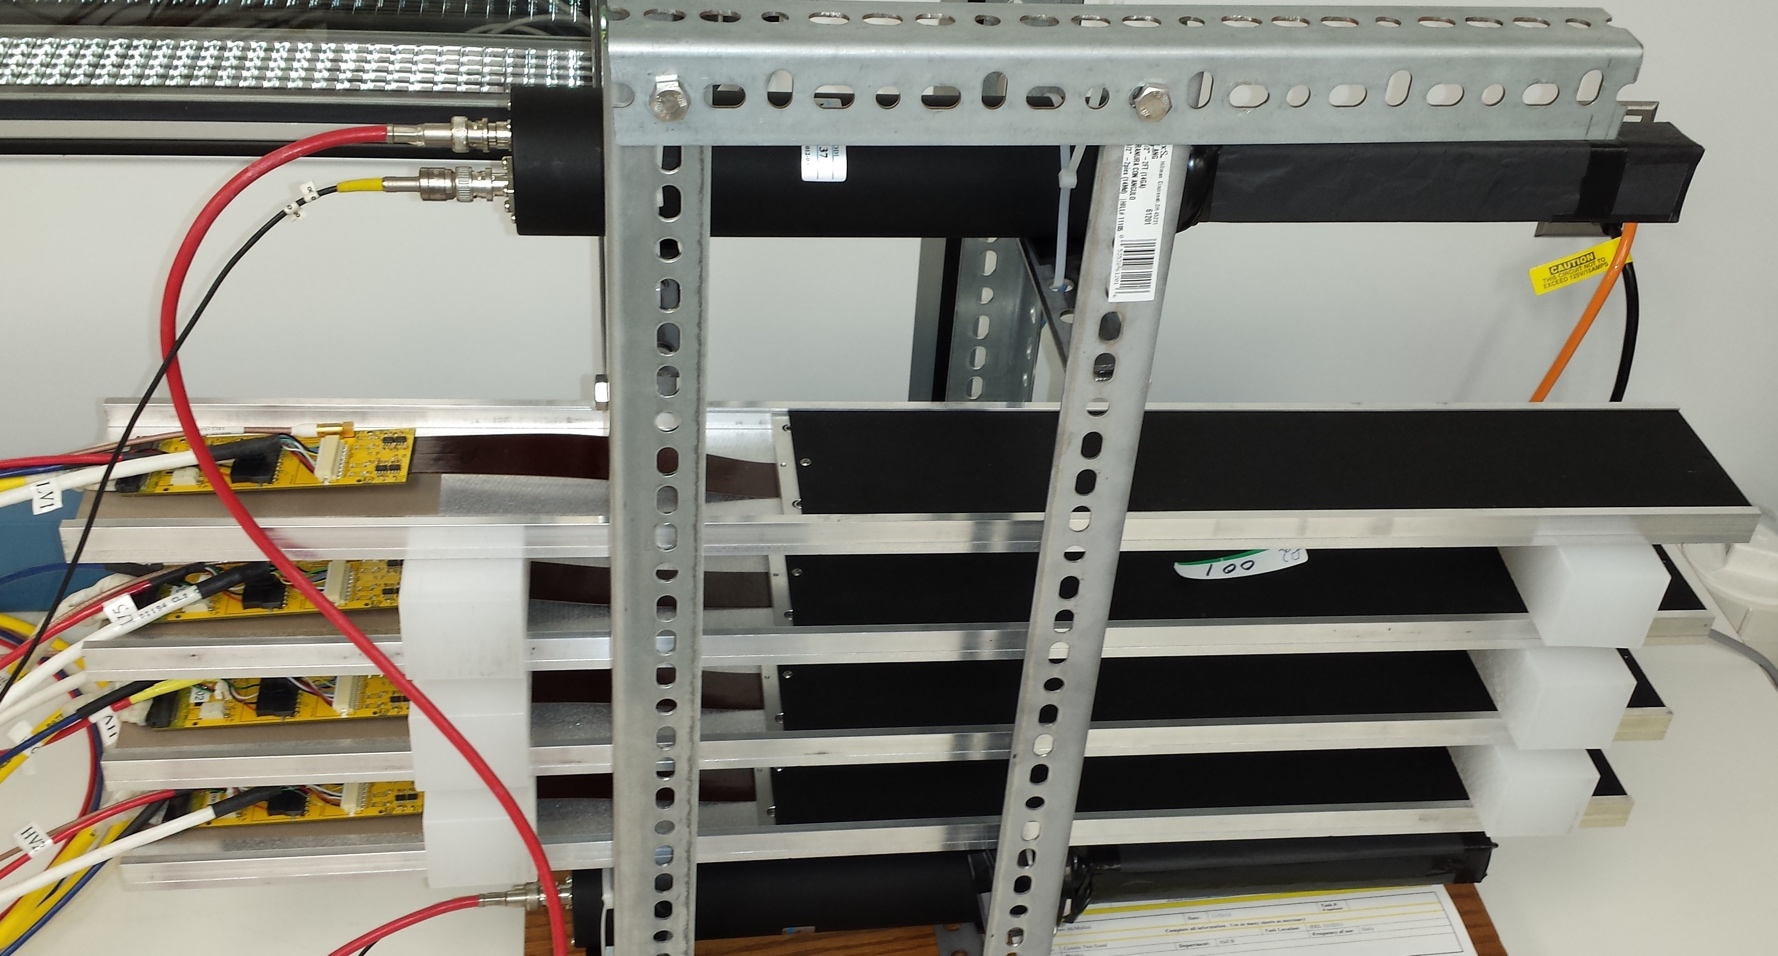
\includegraphics[width=1.0\columnwidth,keepaspectratio]{cosmic-stand.jpg}
\caption{Cosmic test stand.}
\label{fig:cosmic-stand}
\end{figure}

Cosmic data during detector integration in the clean room were taken in the standalone mode using the self triggering feature of the FSSR2 readout chip in coincidence logic. VSCM boards reading the SVT modules located at the top and bottom halves of the horizontally placed barrel provided the trigger signals via signal distribution of two VXS crates. The coincidence of  signals from the trigger interface boards of both crates was taken as the cosmic trigger. The response of the channels was uniform, and performance results obtained during tracker integration were confirmed. The angular distribution of the cosmic muons reconstructed in the SVT is shown in Fig.~\ref{fig:track-phi-theta}.

\begin{figure}[hbt] 
\centering 
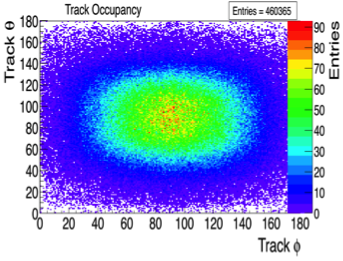
\includegraphics[width=1.0\columnwidth,keepaspectratio]{track-phi-theta.png}
\caption{Angular distribution of the cosmic muons reconstructed in the SVT.}
\label{fig:track-phi-theta}
\end{figure}

After installation of the SVT in the hall and checkout of detector services and readout system, a trigger from the CTOF detector was used to collect cosmic data for the CLAS12 central detector. A cosmic muon reconstructed in the central detector is shown in Fig.~\ref{fig:cd-cosmic-event}. The SVT is the inner detector, surrounded by the BMT, the CTOF, and the CND. Yellow circles represent crosses (matched hits on both sides of the module) in the SVT and green circles correspond to the clusters in the Micromegas detector. Both tracking detectors have the same number of layers. The SVT has small angle stereo strips on the two sides of a module, and the BMT has interleaving layers of the strips along the beam axis and arcs at the fixed radii. Between the physics data taking runs more cosmic trigger data were collected for calibration and performance studies.  A hit map for the SVT channels during the cosmic run is shown in Fig.~\ref{fig:cosmic-hitmap-svt}. Several sensors were under-depleted, visible on the plot as channels with higher occupancy. Lower hit occupancy on the right side of the map is due to the shorter strips at this side of the sensors. 

\begin{figure}[hbt] 
\centering 
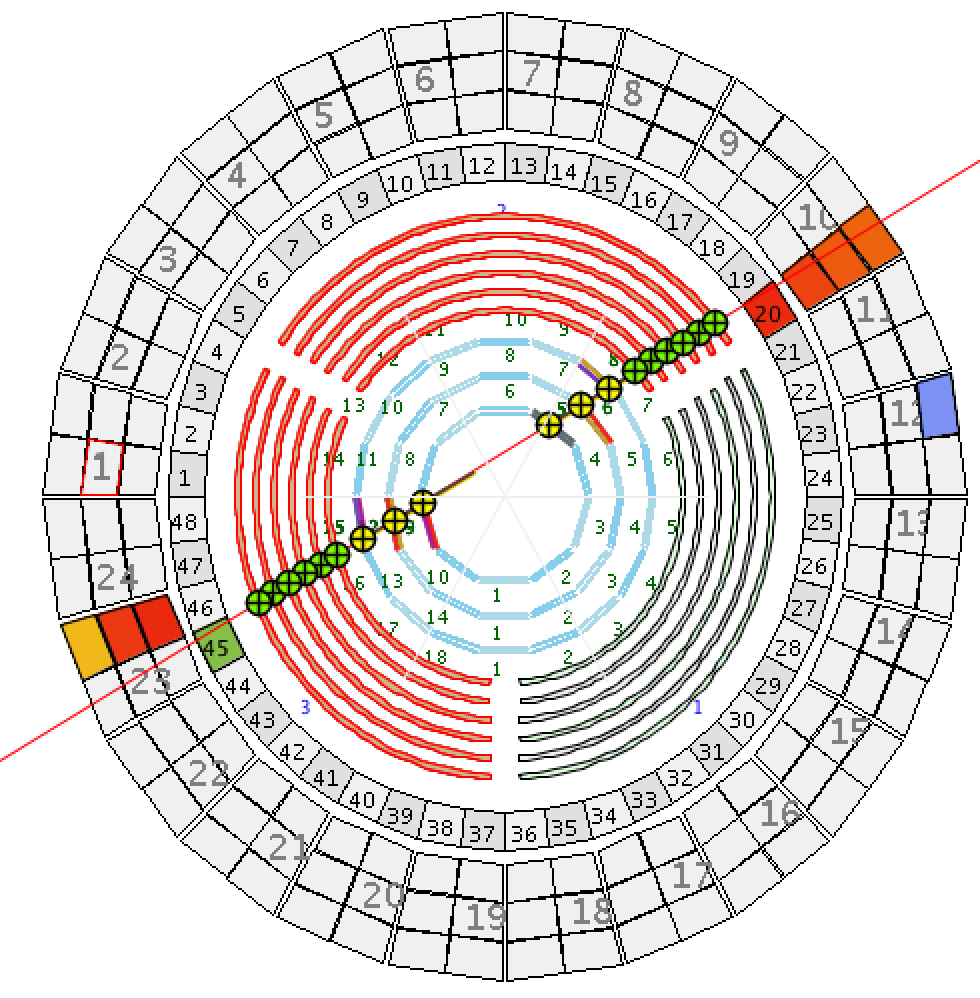
\includegraphics[width=0.8\columnwidth,keepaspectratio]{cd-cosmic-event.png}
\caption{Cosmic muon reconstructed in the CLAS central detector.}
\label{fig:cd-cosmic-event}
\end{figure}

\begin{figure}[hbt] 
\centering 
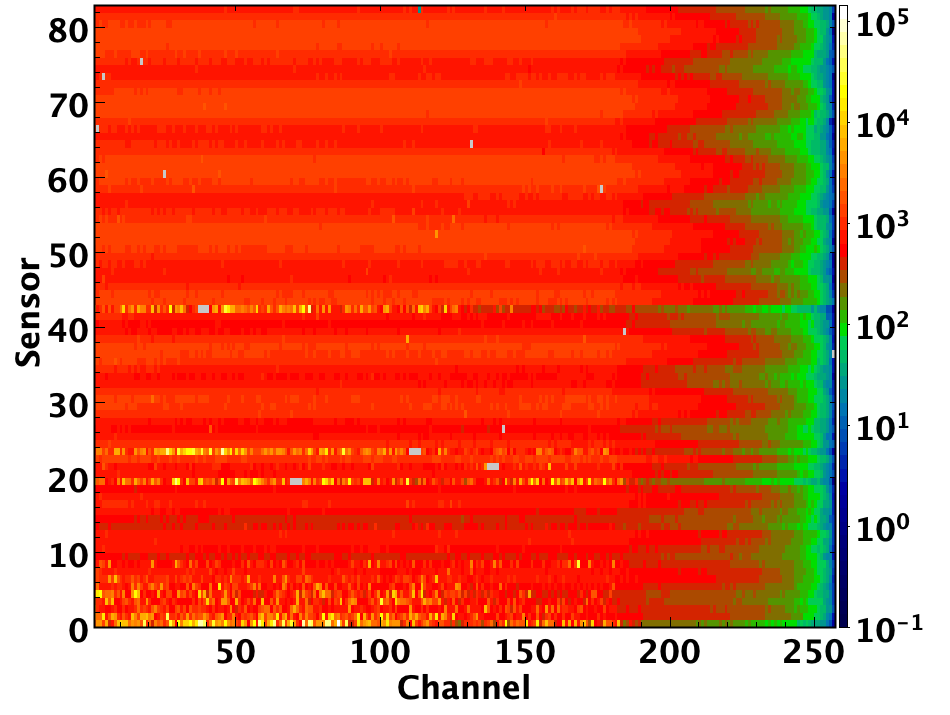
\includegraphics[width=1.0\columnwidth,keepaspectratio]{cosmic-hitmap-svt.png}
\caption{Monitoring SVT hit map during a cosmic run showing module vs. strip number.}
\label{fig:cosmic-hitmap-svt}
\end{figure}

The charge sharing among two adjacent strips was studied using using the $\eta$-function, defined for the 2-strip clusters as the ratio of the pulse height of the left strip to the pulse height of the cluster. Fig.~\ref{fig:eta-function} shows the  $\eta$-function obtained from the measurement of on-track clusters from the cosmic muons. The granularity of the pulse height after the digitization is coarse due to the 3-bit ADC of the readout chip. There is a pronounced peak in the center between the two readout strips where all the charge is collected by the intermediate strip. Because of capacitive coupling, signals on these intermediate strips are partially transferred to the readout strips.

\begin{figure}[hbt] 
\centering 
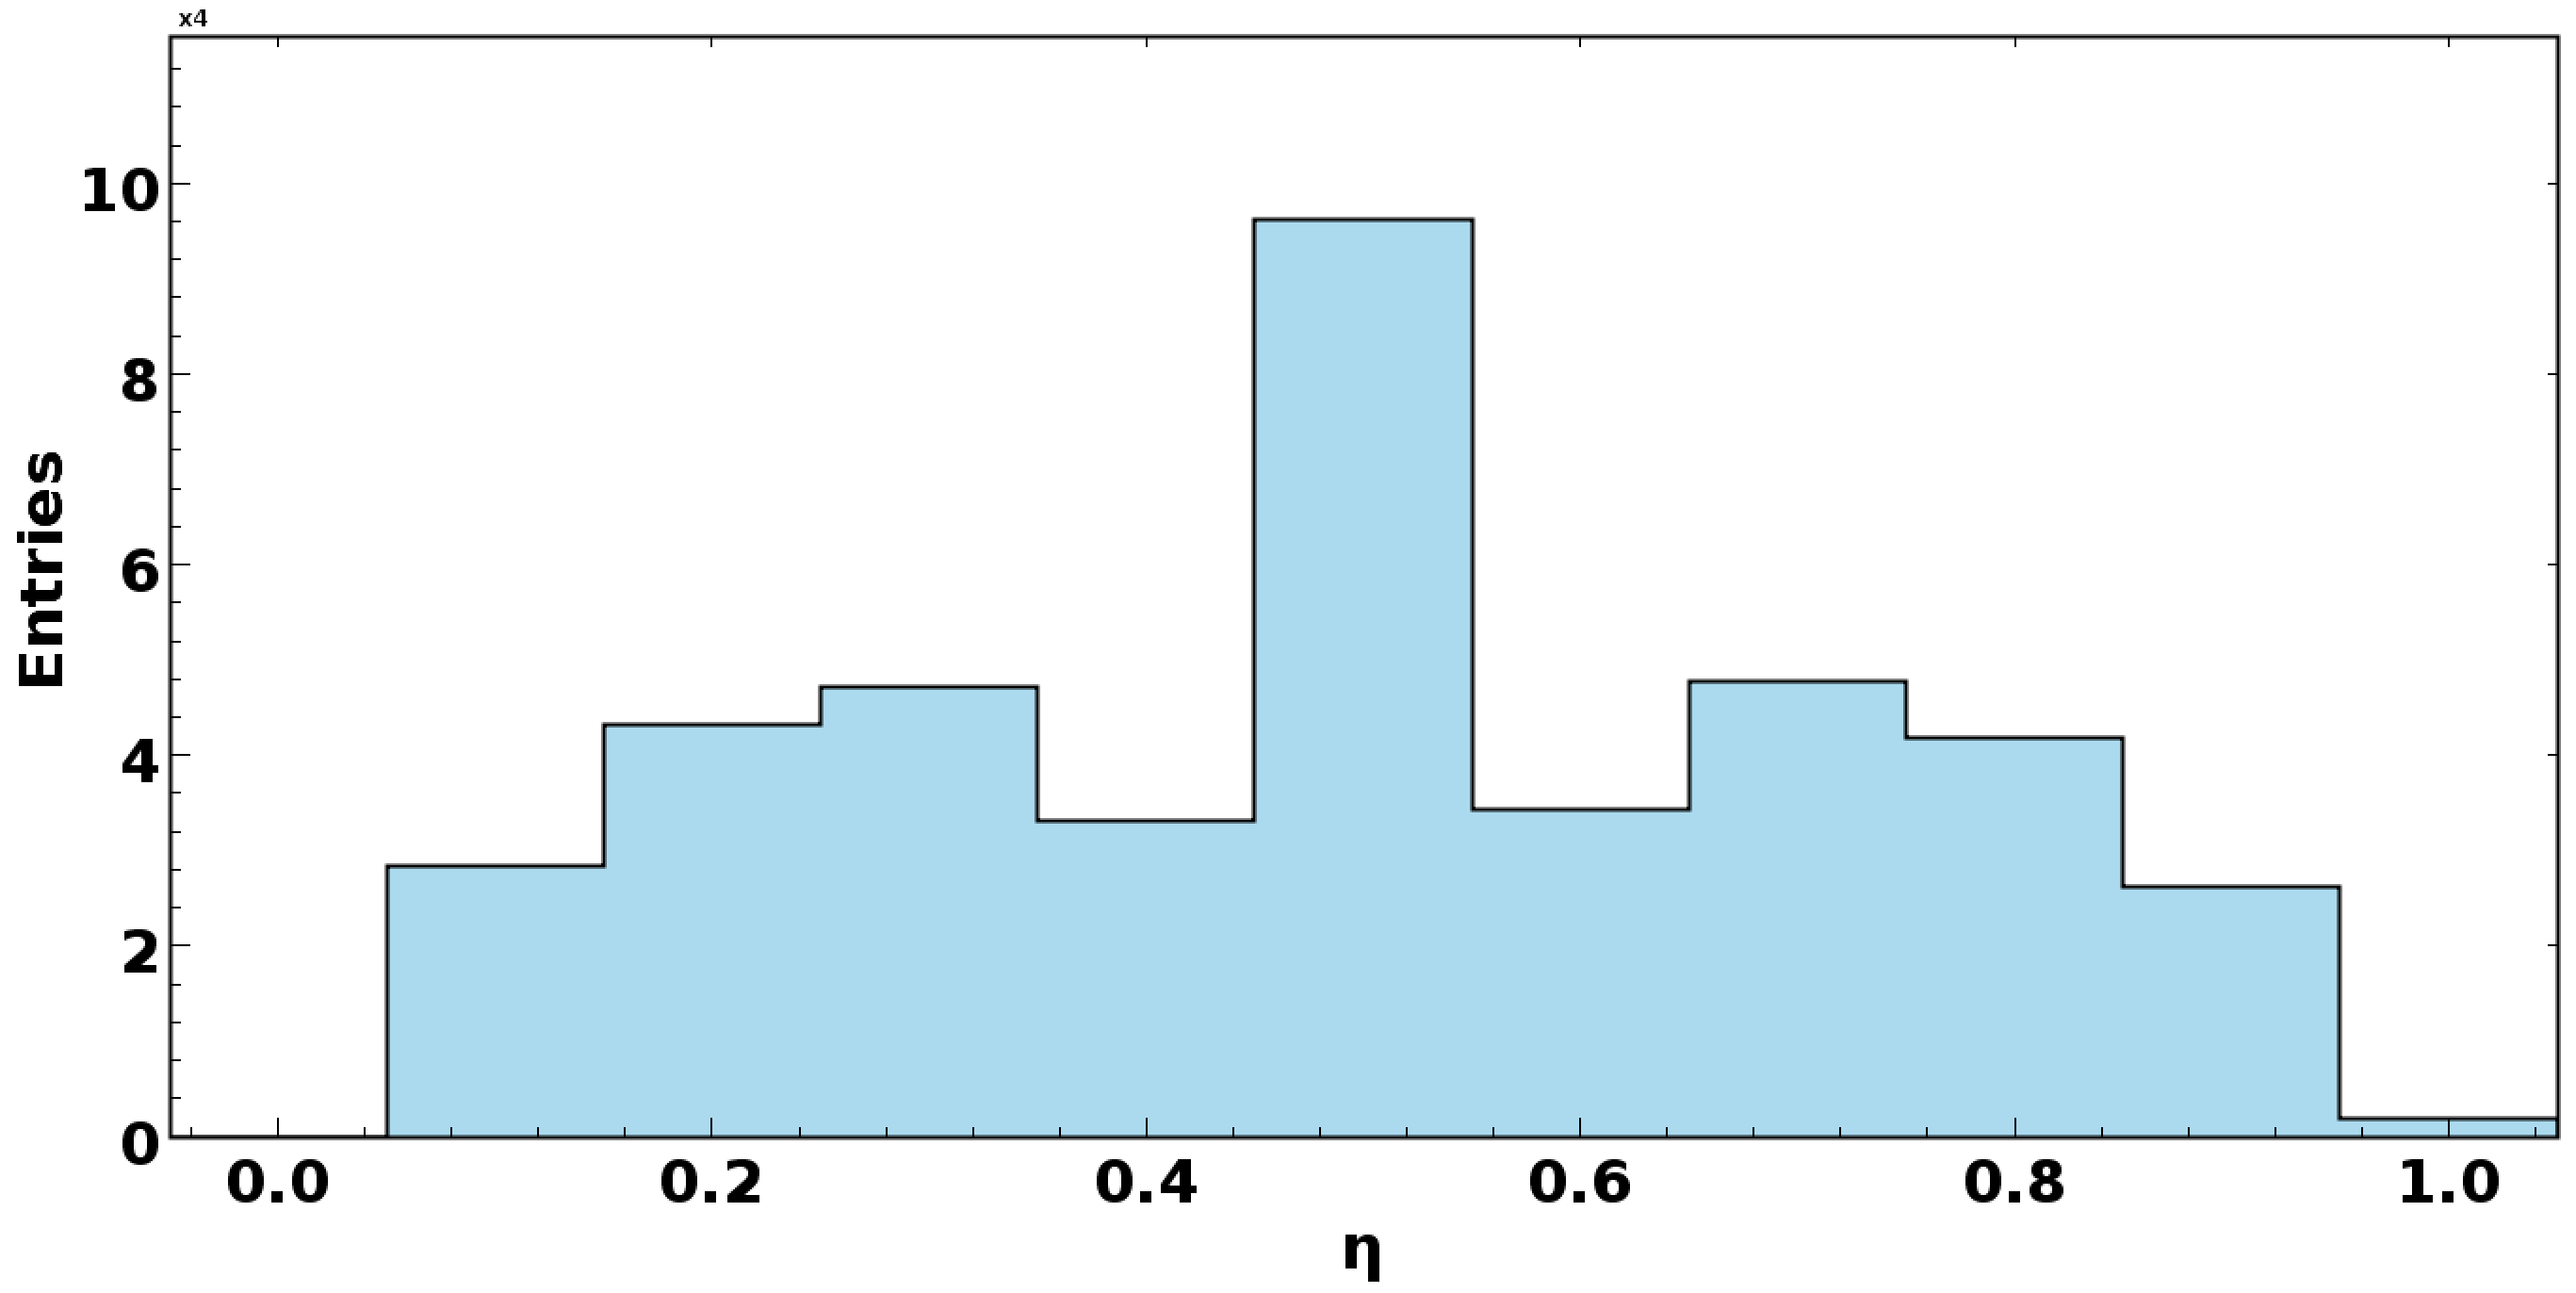
\includegraphics[width=1.0\columnwidth,keepaspectratio]{eta-function.png}
\caption{$\eta$-function for the two-strip clusters.}
\label{fig:eta-function}
\end{figure}

Strip multiplicity of the clusters (cluster size) in the cosmic run is shown in Fig.~\ref{fig:cluster-size}. The size of the clusters is lowest in the innermost region and is increasing with radius due to a larger local track angle (the tracks, triggered by the CTOF, crossing the barrel far from the beam line). The results are in agreement with simulations and the data on the charge sharing among adjacent readout strips obtained with the laser.

\begin{figure}[hbt] 
\centering 
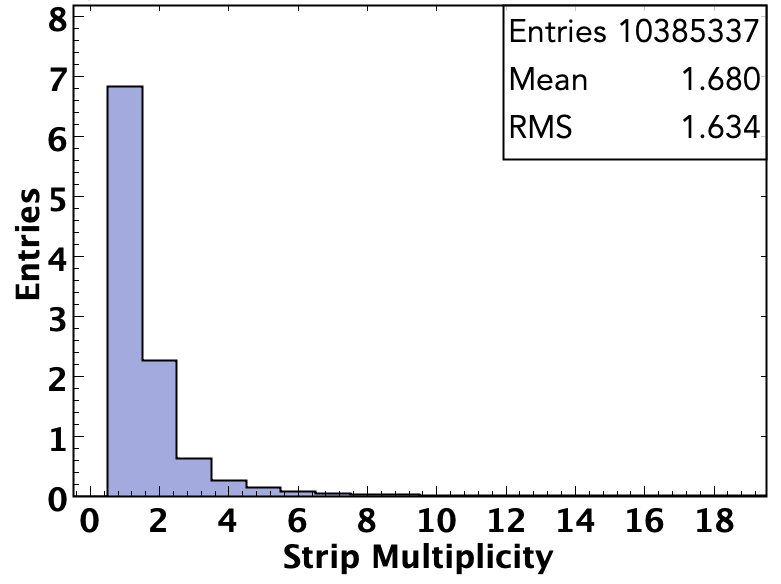
\includegraphics[width=1.0\columnwidth,keepaspectratio]{cluster-size.png}
\caption{Strip multiplicity of the clusters in the cosmic run.}
\label{fig:cluster-size}
\end{figure}

Cosmic muons are an important source for calibration and alignment. Their trajectories are sensitive to misalignments of different tracker parts. The cosmic muons significantly improve the alignment precision. A preliminary alignment of the SVT was done using the sample of several millions of the cosmic muon tracks taken without solenoid magnetic field. With exception of the modules located at the shallow angle to the vertical axis, the acquired sample provided adequate statistics of the tracks to extract the misalignment data. The tracks crossing the sensors at large inclination angles and low energy tracks subject to multiple scattering were rejected. Additional requirement on the $\chi^2$ per degree of freedom of the track fit was applied to reject tracks effected by the outlier hits. The spacial residuals before (blue) and after (red) the alignment procedure (see Fig.~\ref{fig:alignment}) are shown. Only the shifts in the sensor plane were taken into account in the alignment procedure for this plot. Validation of alignment procedures was performed on Monte Carlo simulation and cosmic data.

\begin{figure}[hbt] 
\centering 
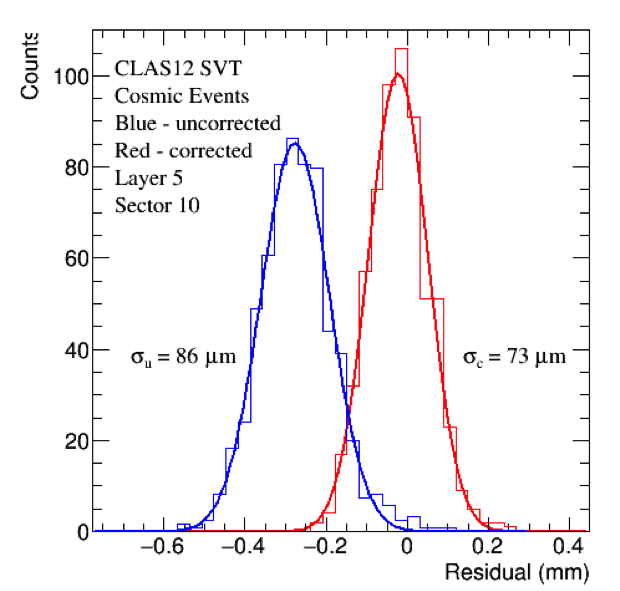
\includegraphics[width=1.0\columnwidth,keepaspectratio]{alignment.png}
\caption{Residuals for one of the SVT sensors before (blue) and after (red) alignment.}
\label{fig:alignment}
\end{figure}

\subsection{Commissioning with beam}

Performance of the SVT module has been studied at Fermilab in a beam test with 120 GeV protons. SVT module in the plastic carrier box was mounted vertically behind the CMS pixel beam telescope (8 planes, $\approx$6 $\mu$m track position uncertainty, 2 $\times$ 2 cm active area), used as the trigger and the tracker. Beam test setup is shown in Fig.~\ref{fig:beam-test}. Production SVT DAQ has been exercised at different event rates. Event block mode has been tested up to 100 k protons per 4 sec spill with no busy time. Signal-to-Noise ratio was in agreement with results with radioactive sources and cosmic muons. Measured cluster charge distribution is shown in Fig.~\ref{fig:cluster-charge-protons}. Several millions triggers have been taken at different discriminator thresholds.  Expected position resolution of the silicon sensors was confirmed. 

\begin{figure}[hbt] 
\centering 
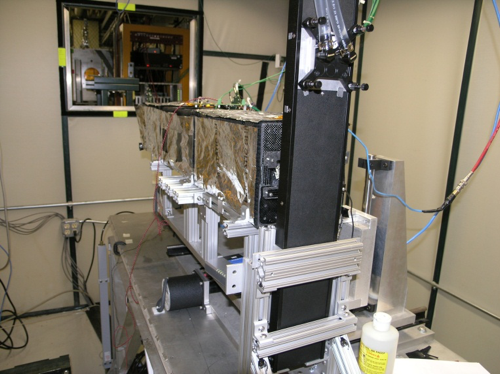
\includegraphics[width=1.0\columnwidth,keepaspectratio]{beam-test.png}
\caption{Beam test setup.}
\label{fig:beam-test}
\end{figure}

\begin{figure}[h] 
\centering 
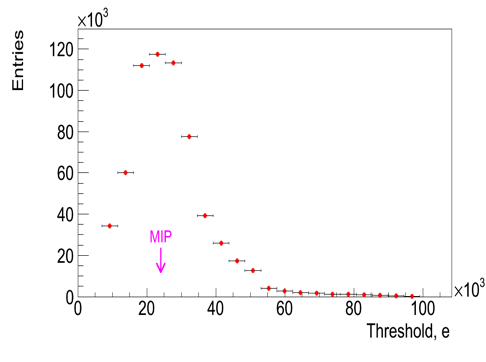
\includegraphics[width=1.0\columnwidth,keepaspectratio]{cluster-charge-protons.png}
\caption{Cluster charge distribution from 120 GeV protons.}
\label{fig:cluster-charge-protons}
\end{figure}

The front-end electronics performance and noise occupancy of the detector were studied during physics data taking. No interference with other CLAS12 subsystems were found. The data quality and detector operational stability  were verified with both online and offline monitoring packages. There were occasional FSSR2 chip latch-ups observed after the start of a new run. These latch-ups were traced by improper configuration of the chips and fixed by adding additional resets to the run start sequence.

\begin{figure}[h] 
\centering 
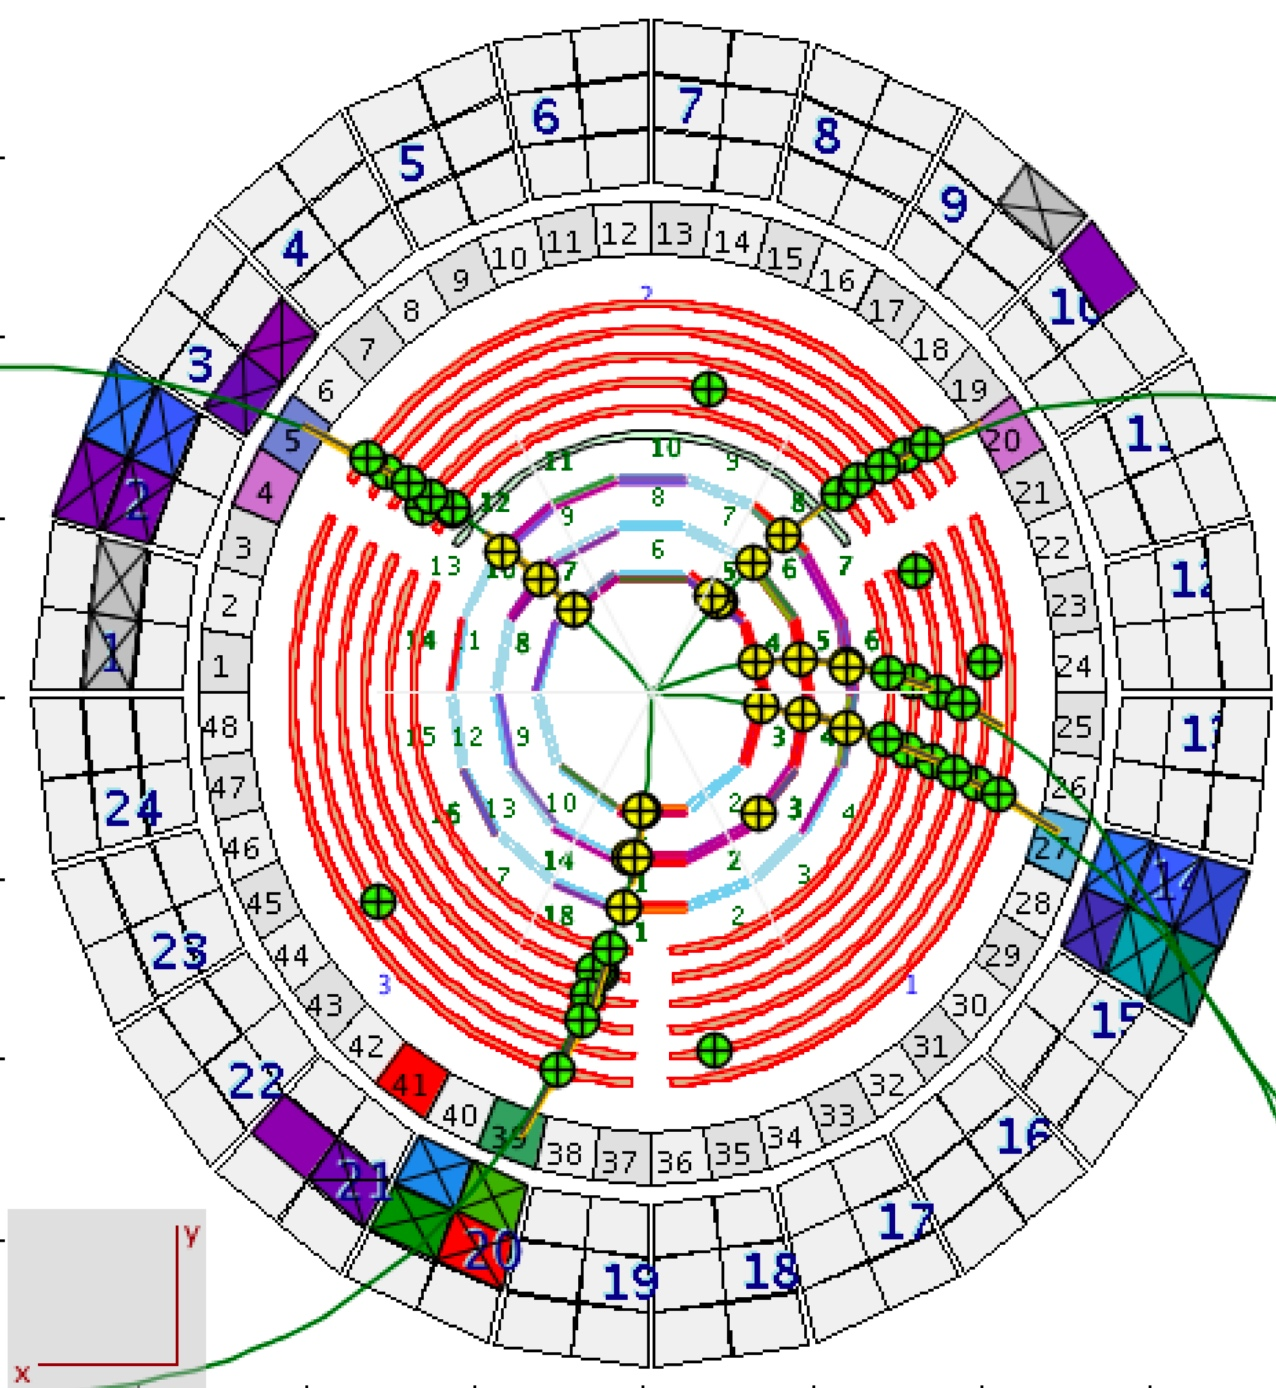
\includegraphics[width=0.8\columnwidth,keepaspectratio]{cd-tracks.jpg}
\caption{Multi-track event reconstructed in the CLAS12 central detector during a physics run.}
\label{fig:cd-tracks}
\end{figure}

Tracks reconstructed in the CLAS12 central detector during a physics run are shown in Fig.~\ref{fig:cd-tracks}. The level-1 trigger latency is finely tuned to match the CLAS12 trigger delays. Single Event Monitor (SEM) error checking implemented in the VSCM firmware allows real-time monitoring of the readout errors induced by the radiation. Relatively minor single event upsets were recorded in the SVT readout electronics with no latch-ups or single event burn-outs observed. The SEM recorded events are correlated with beam conditions in the experimental hall during the run. SVT readout and power supply crates did not require rebooting. No readout or data corruption issues were observed \cite{SEENOTE}. 

\begin{figure}[htb] 
\centering 
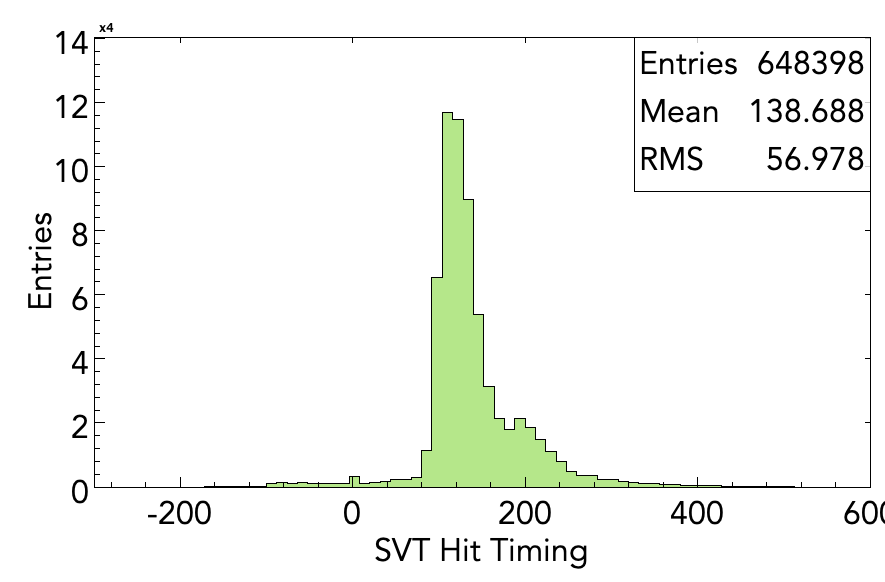
\includegraphics[width=1.0\columnwidth,keepaspectratio]{svt-hit-timing.png}
\caption{SVT hit timing referenced to the CTOF time in a physics run with the hydrogen target.}
\label{fig:svt-hit-timing}
\end{figure}

FSSR2 readout chip does not provide the timing information from the hit. Reading the time stamp associated with a hit was implemented in the VSCM board. The time stamp is synchronized with the "Got Hit" pulse from the chip when the pulse height reaches the threshold set for the first discriminator of the ADC. Timing of the SVT hits referenced to the CTOF timing are shown in Fig.~\ref{fig:svt-hit-timing}. The data correspond to the time difference between the SVT and the CTOF time stamps for the SVT hits which were associated with a track. Applying a cut on this difference can be  used to remove background and noise hits in the track seeding algorithm.

Radiation induced energy levels in the middle of the band gap are causing an increase of thermally generated electron-hole pairs. The sensor leakage current increases with the absorbed flux:

\begin{equation} \Delta I_R = \alpha \Phi \label{eq:leakage-fluence},
\end{equation}

where $\Phi$ is the particle fluence and $\alpha \approx$ 4$\cdot$10$^{-17}$ A/cm~\cite{DIERLAMMTHESIS}. The increased leakage current is increasing the noise and heating up the sensor, which, in turn, will further increase the leakage current. When the temperature increases beyond a critical temperature where the cooling can not maintain a stable temperature this will result in thermal runaway. After accumulating a large hadron fluence, the SVT requires low temperature operation to avoid thermal runaway induced by the sensor leakage current. Fig.~\ref{fig:thermal-runaway} shows thermal runaway in the 2 innermost layers of the SVT received the highest radiation dose. Leakage currents in other layers were stable. The monitoring data were taken after a physics run with liquid hydrogen target, when there was no beam in the hall for extended time. The leakage currents became stable when the coolant temperature was decreased.

\begin{figure}[hbt] 
\centering 
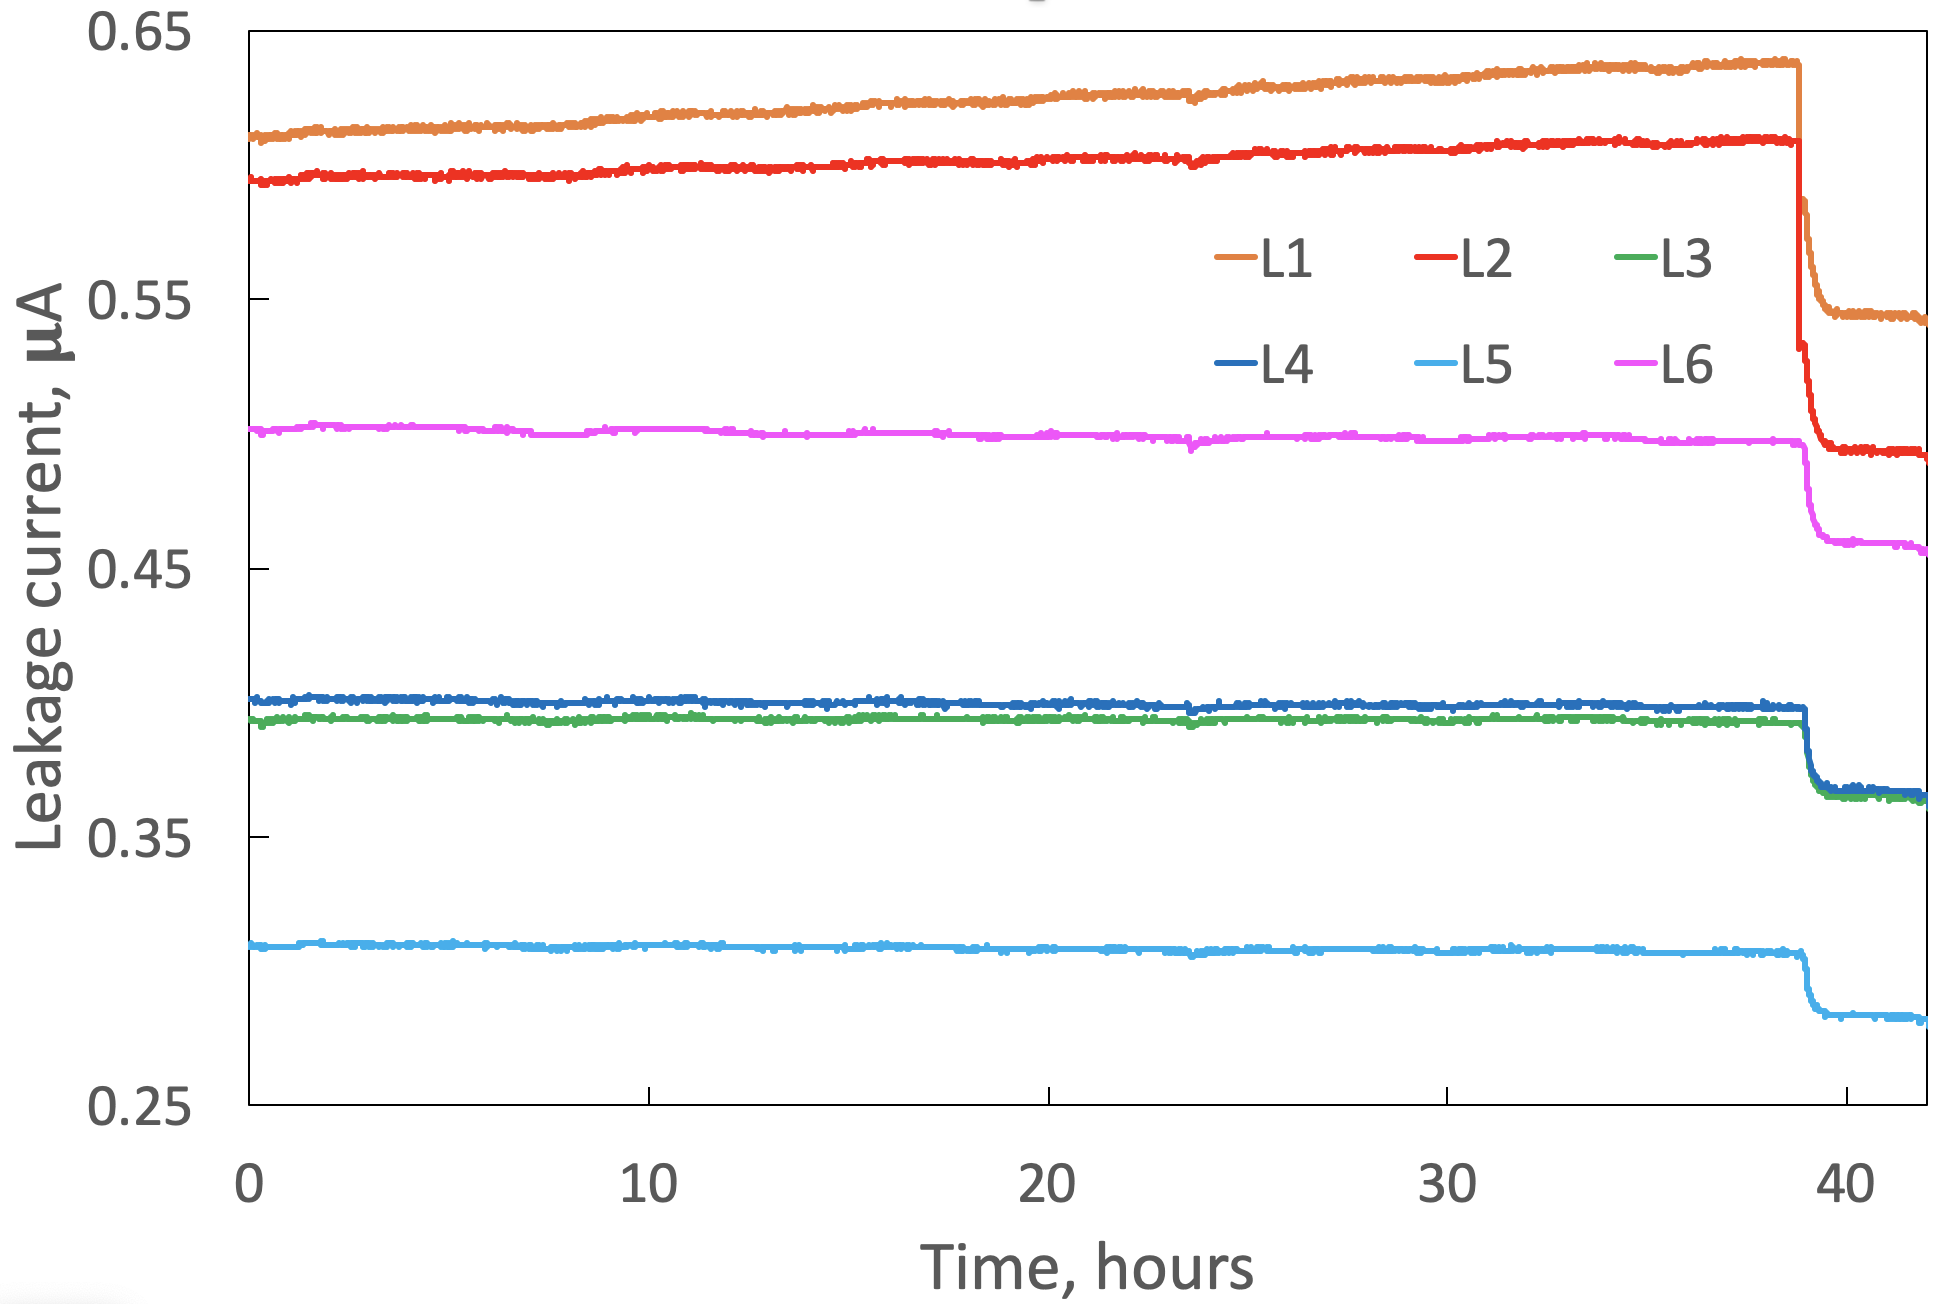
\includegraphics[width=1.0\columnwidth,keepaspectratio]{thermal-runaway.png}
\caption{Thermal runaway in the SVT inner layers (L1 and L2).}
\label{fig:thermal-runaway}
\end{figure}

Fig.~\ref{fig:leakage-layers-deuterium} shows monitoring plots for the average sensor leakage currents in the SVT layers during the data taking with liquid deuterium target. For the first few hours in the time period shown there was no beam in the hall and the currents were stable. Currents in all the layers are increasing with time when beam is present. The jumps in the leakage current of a layer between two values are related to the beam trips. The largest difference between beam-on and beam-off levels and the rate of current increase is in the inner layers. The data were taken at 50 nA beam current. 

\begin{figure}[hbt] 
\centering 
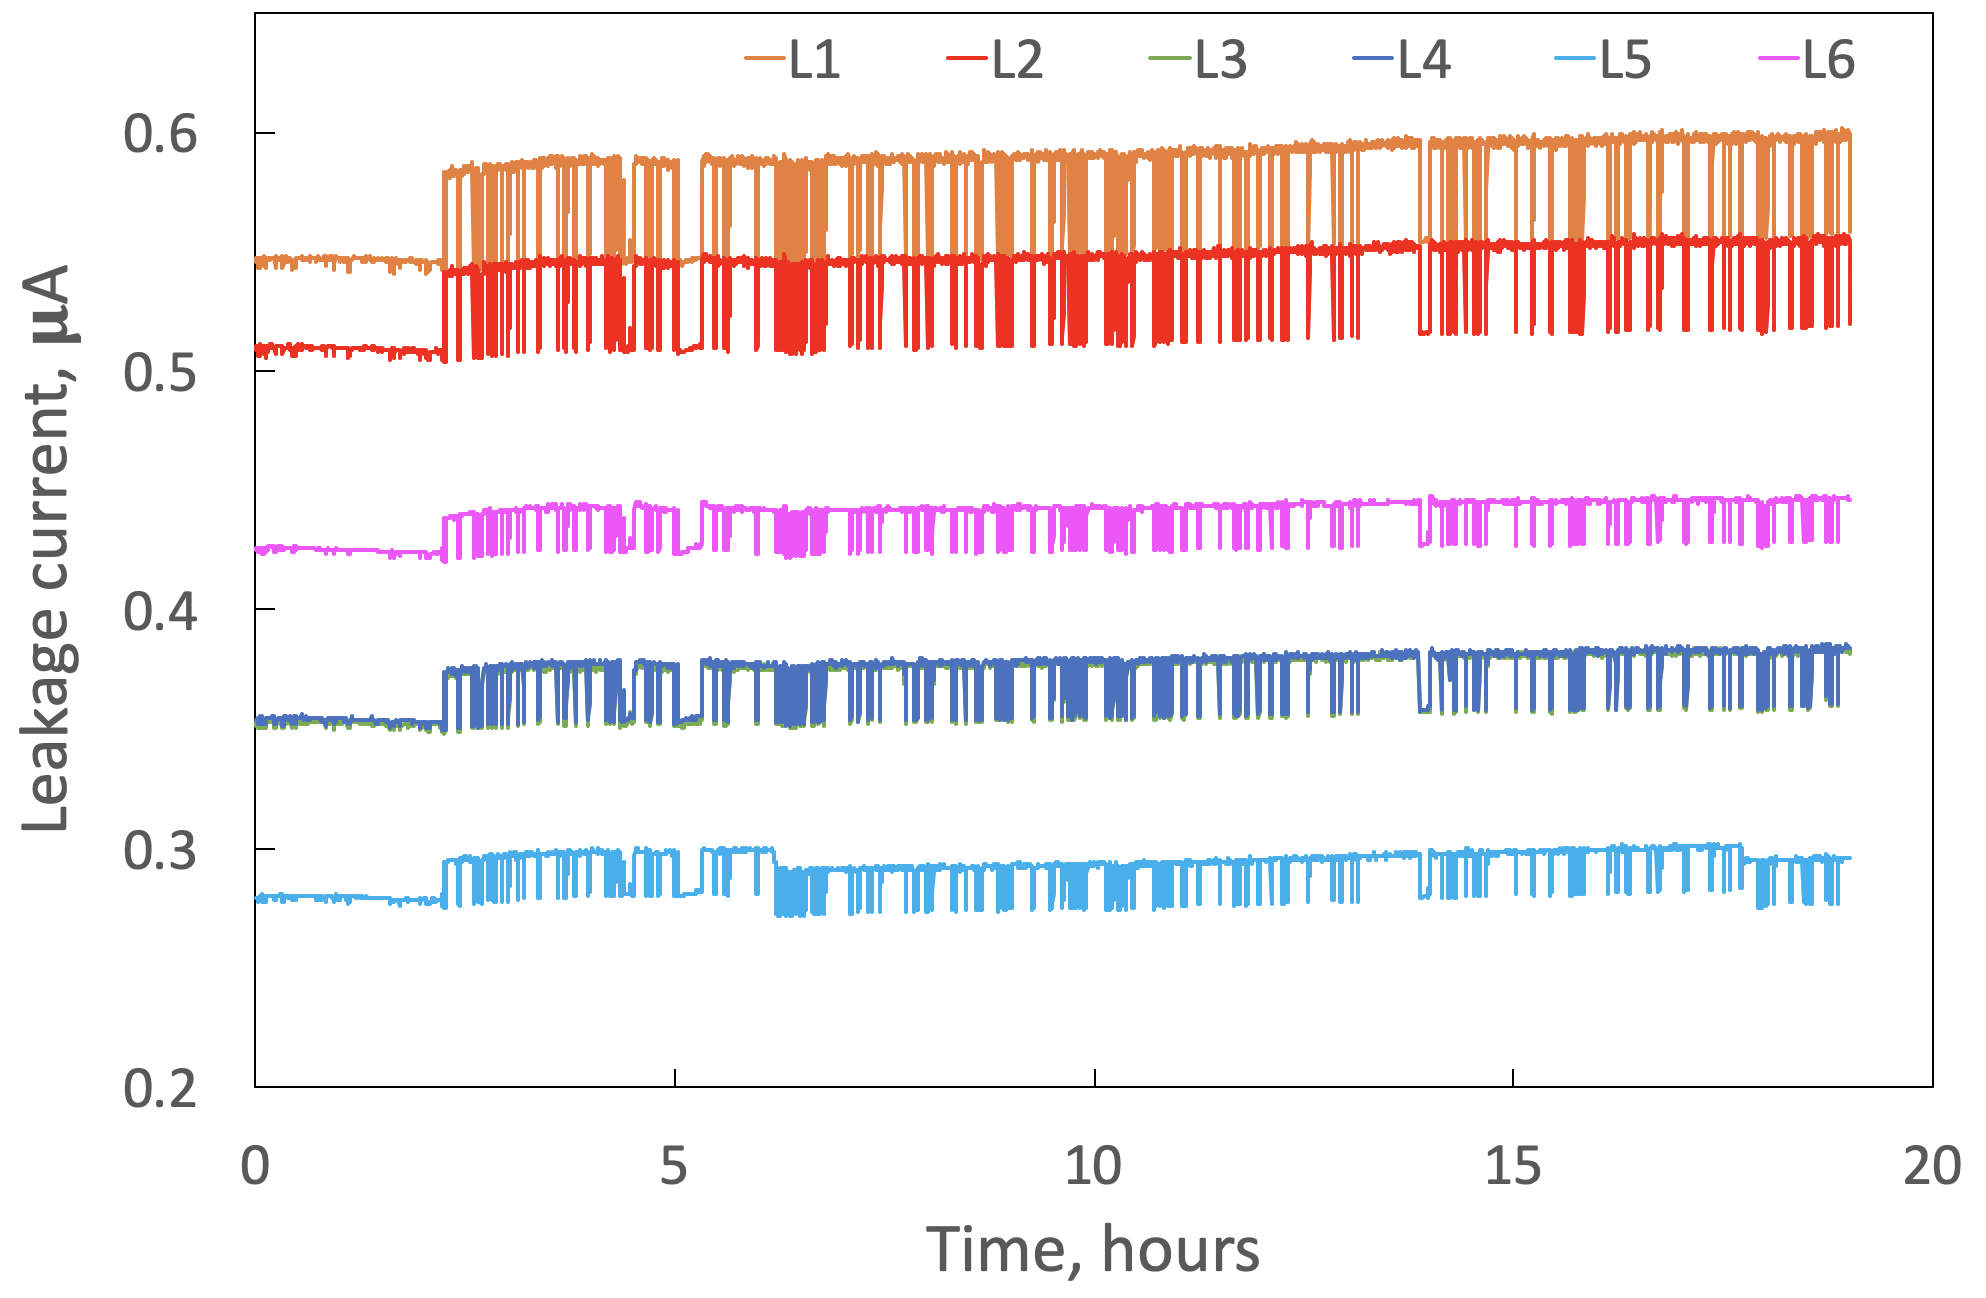
\includegraphics[width=1.0\columnwidth,keepaspectratio]{leakage-layers-deuterium.png}
\caption{Monitoring plots of the sensor leakage currents in the SVT layers during the run with liquid deuterium target.}
\label{fig:leakage-layers-deuterium}
\end{figure}

Comparison of the rates of leakage current increase with different targets is shown in Fig.~\ref{fig:leakage-hydrogen-duterium}. The rate of current increase with liquid deuterium target was about 1 nA per hour. The rate for liquid hydrogen target was 0.06 nA per hour. The data were taken at 50 nA beam current corresponding to the instantaneous luminosity of 0.7~$\times$10$^{35}$cm$^{-2}$s$^{-1}$ per nucleon.

\begin{figure}[hbt] 
\centering 
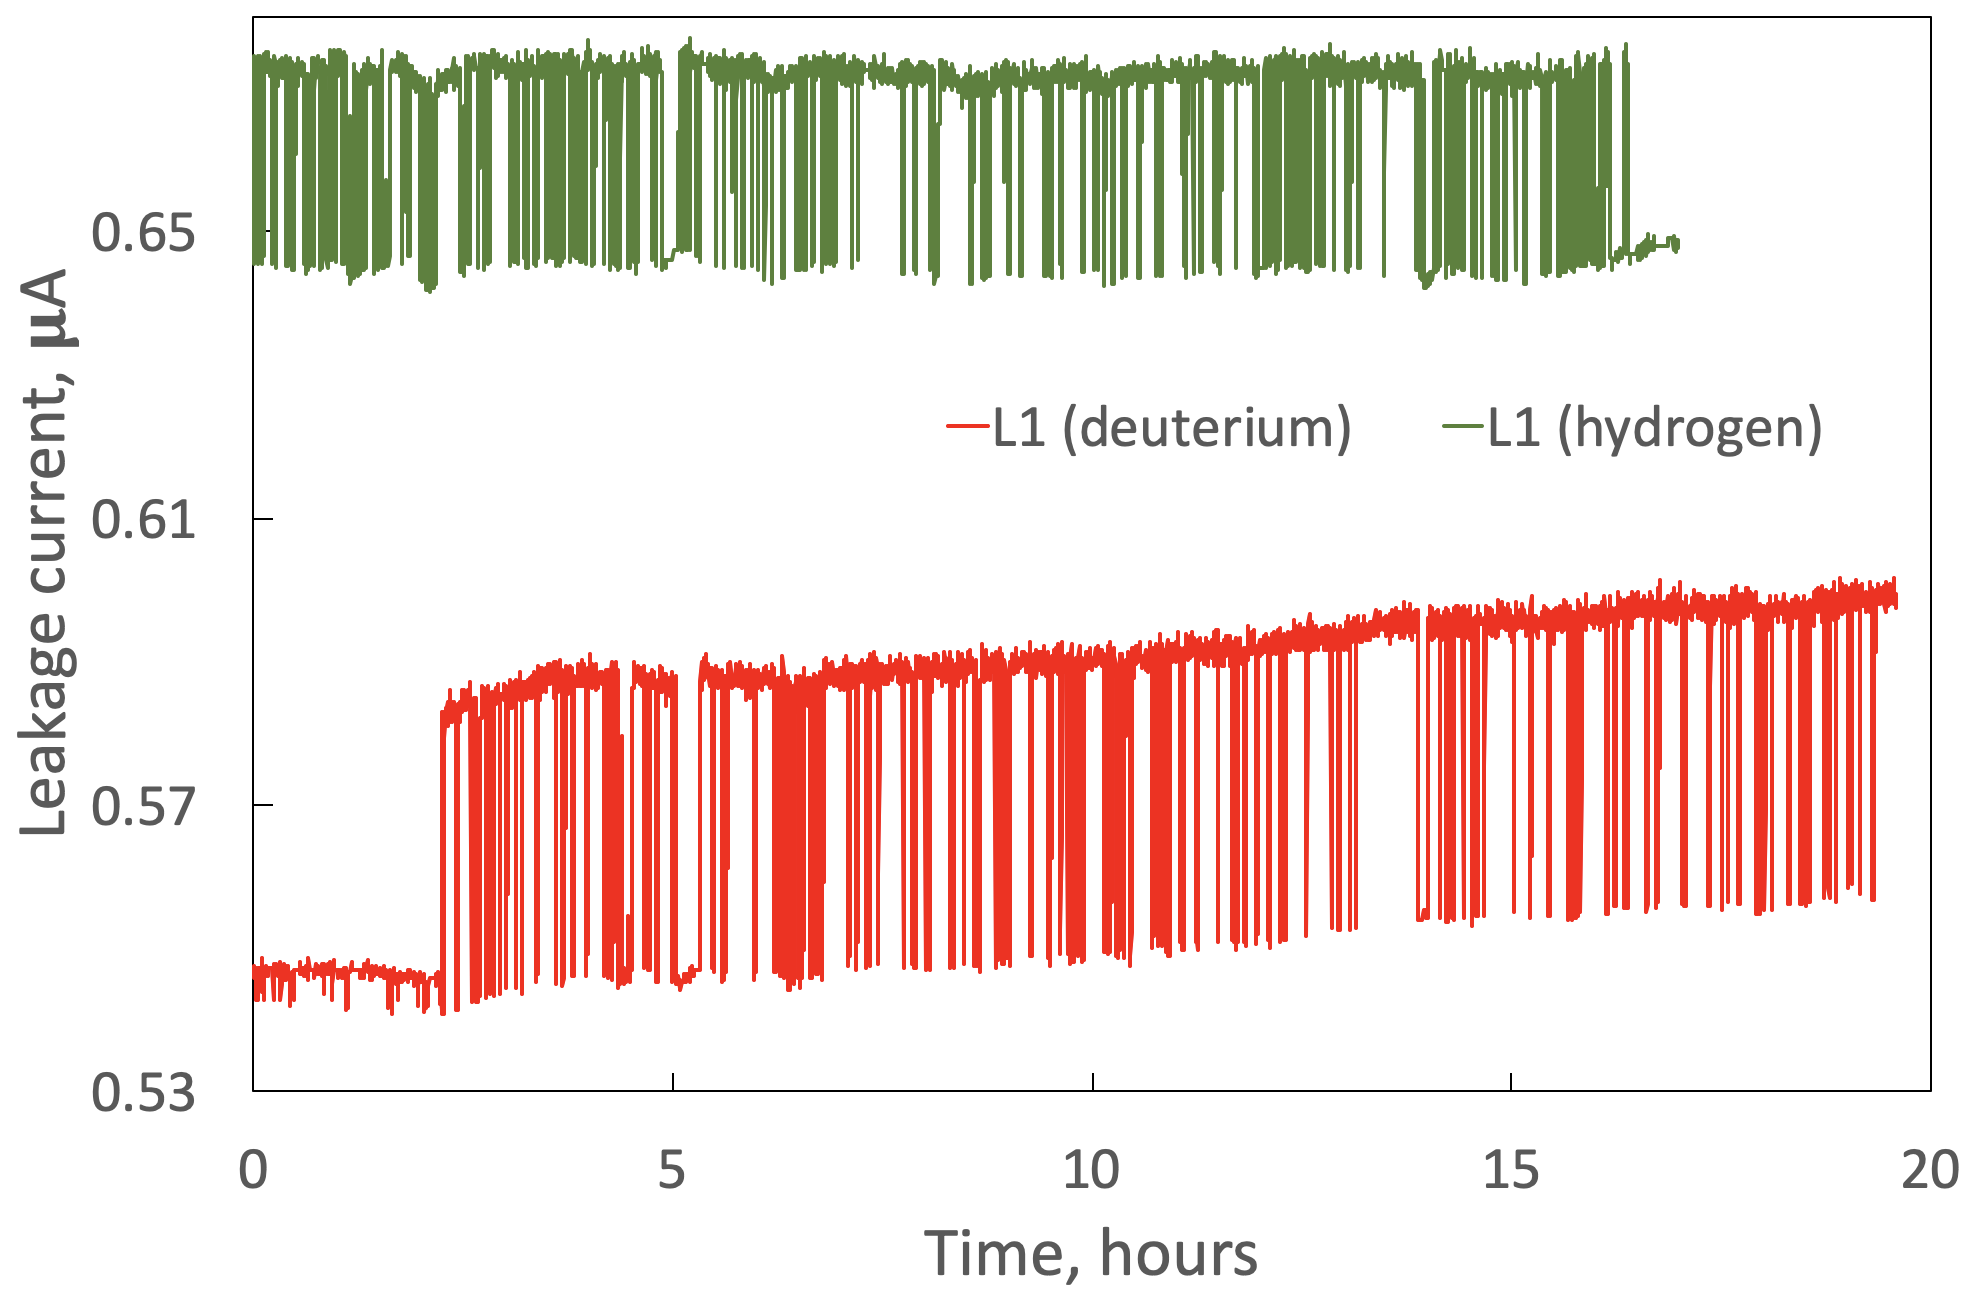
\includegraphics[width=1.0\columnwidth,keepaspectratio]{leakage-hydrogen-duterium.png}
\caption{Average sensor leakage currents in the SVT layer 1 during the runs with hydrogen and deuterium targets.}
\label{fig:leakage-hydrogen-duterium}
\end{figure}

The rate of current increase for the hydrogen target was much smaller.
\begin{figure}[hbt] 
\centering 
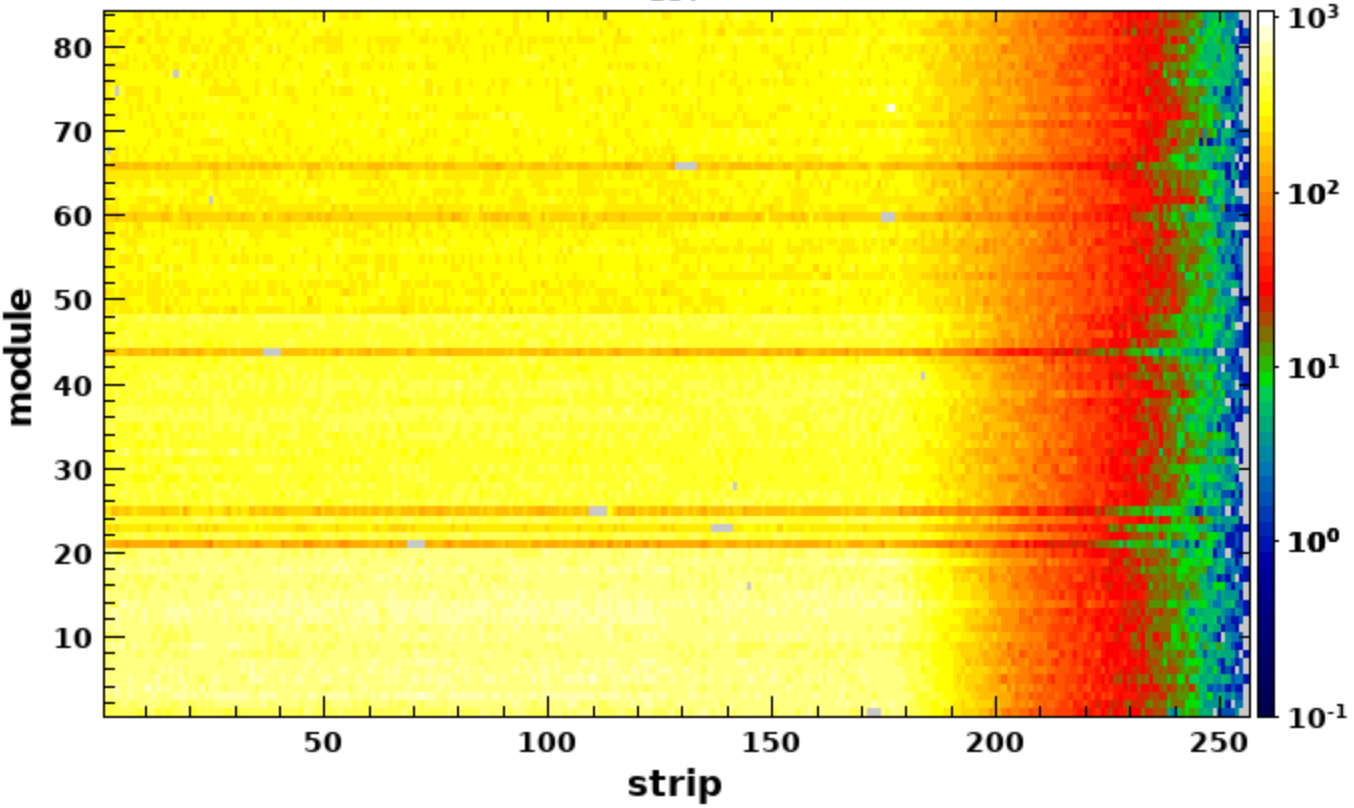
\includegraphics[width=1.0\columnwidth,keepaspectratio]{hit-map-rga.png}
\caption{SVT hit map during a physics run with the hydrogen target.}
\label{fig:hit-map-rga}
\end{figure}

The surface of silicon sensors suffers from the damage due to the ionizing radiation. The damage affects the insulating properties of SiO$_2$ layer between the strips and the aluminum electrodes, collecting the charge generated by the photons and the charged particles. The trapped positive charge is causing accumulation of electrons in the Si/SiO$_2$ interface between the strips, thus decreasing the resistance between the strips and increasing the interstrip capacitance which affects noise performance and degrades the spacial resolution. After a year of running several sensors developed pinholes (the strips with DC current through the damaged dielectric between aluminum strip and implant, resulting in a high current flowing into a channel) observed as groups of adjacent hot channels. The performance of the charge amplifying chip is deteriorated by the high current flowing into a channel. The bias voltage on these sensors has been lowered to reduce noise and abnormally high leakage currents (high occupancy regions on the map). The increased leakage current was reduced by decreasing the detector temperature. The sensors are kept below -10$\degree$C to freeze the reverse annealing interleaved with short periods at room temperature for the beneficial annealing. A hit map of the SVT from a physics run is shown in Fig.~\ref{fig:hit-map-rga}. Sensors with pinholes are seen on the map as darker horizontal lines due to reduced efficiency (under-depleted sensors) with strips of masked hot channels with no hits. 

\begin{figure}[hbt] 
\centering 
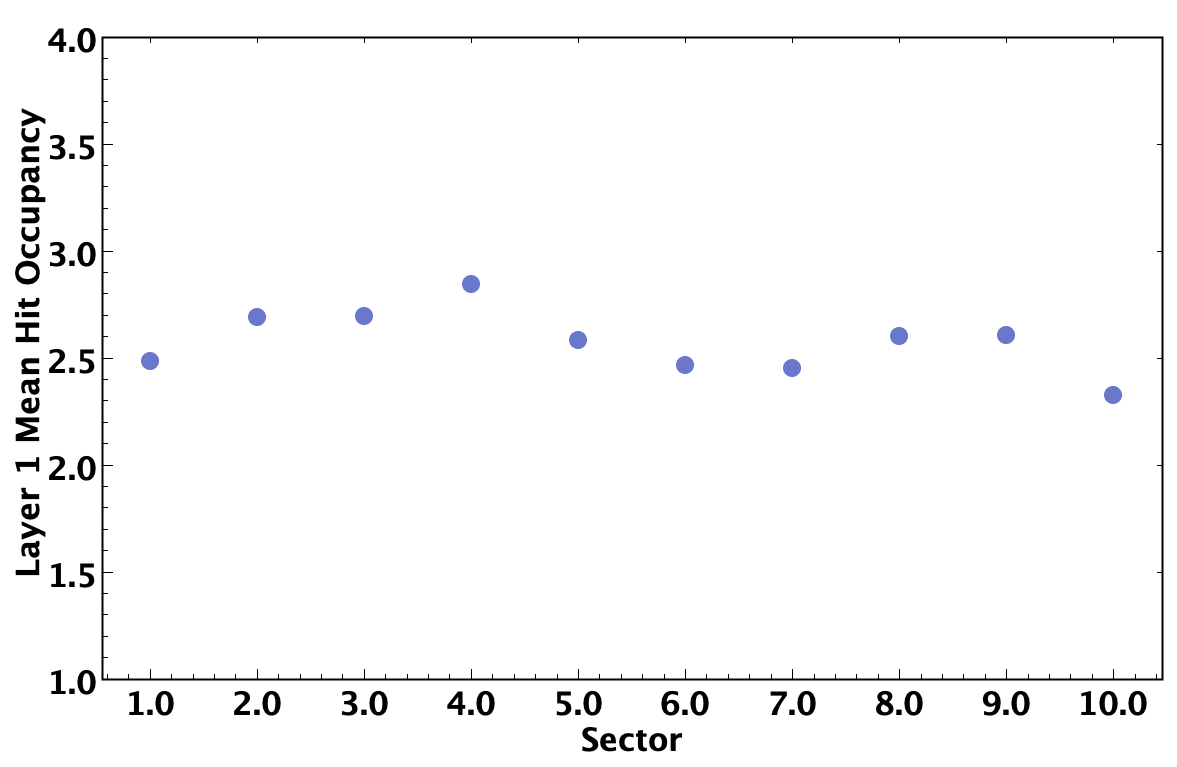
\includegraphics[width=1.0\columnwidth,keepaspectratio]{mean-hit-occupancy.png}
\caption{Mean hit occupancies for the sectors of the innermost SVT layer with hydrogen target at 50 nA beam current.}
\label{fig:mean-hit-occupancy}
\end{figure}

Fig.~\ref{fig:mean-hit-occupancy} shows average hit occupancy per event in the innermost SVT layer for the data taken with hydrogen target at nominal beam current of 50 nA. The hits are uniformly distributed among the sectors with occupancies close to 1$\%$ (each sensor has 256 strips).

\begin{figure}[hbt] 
\centering 
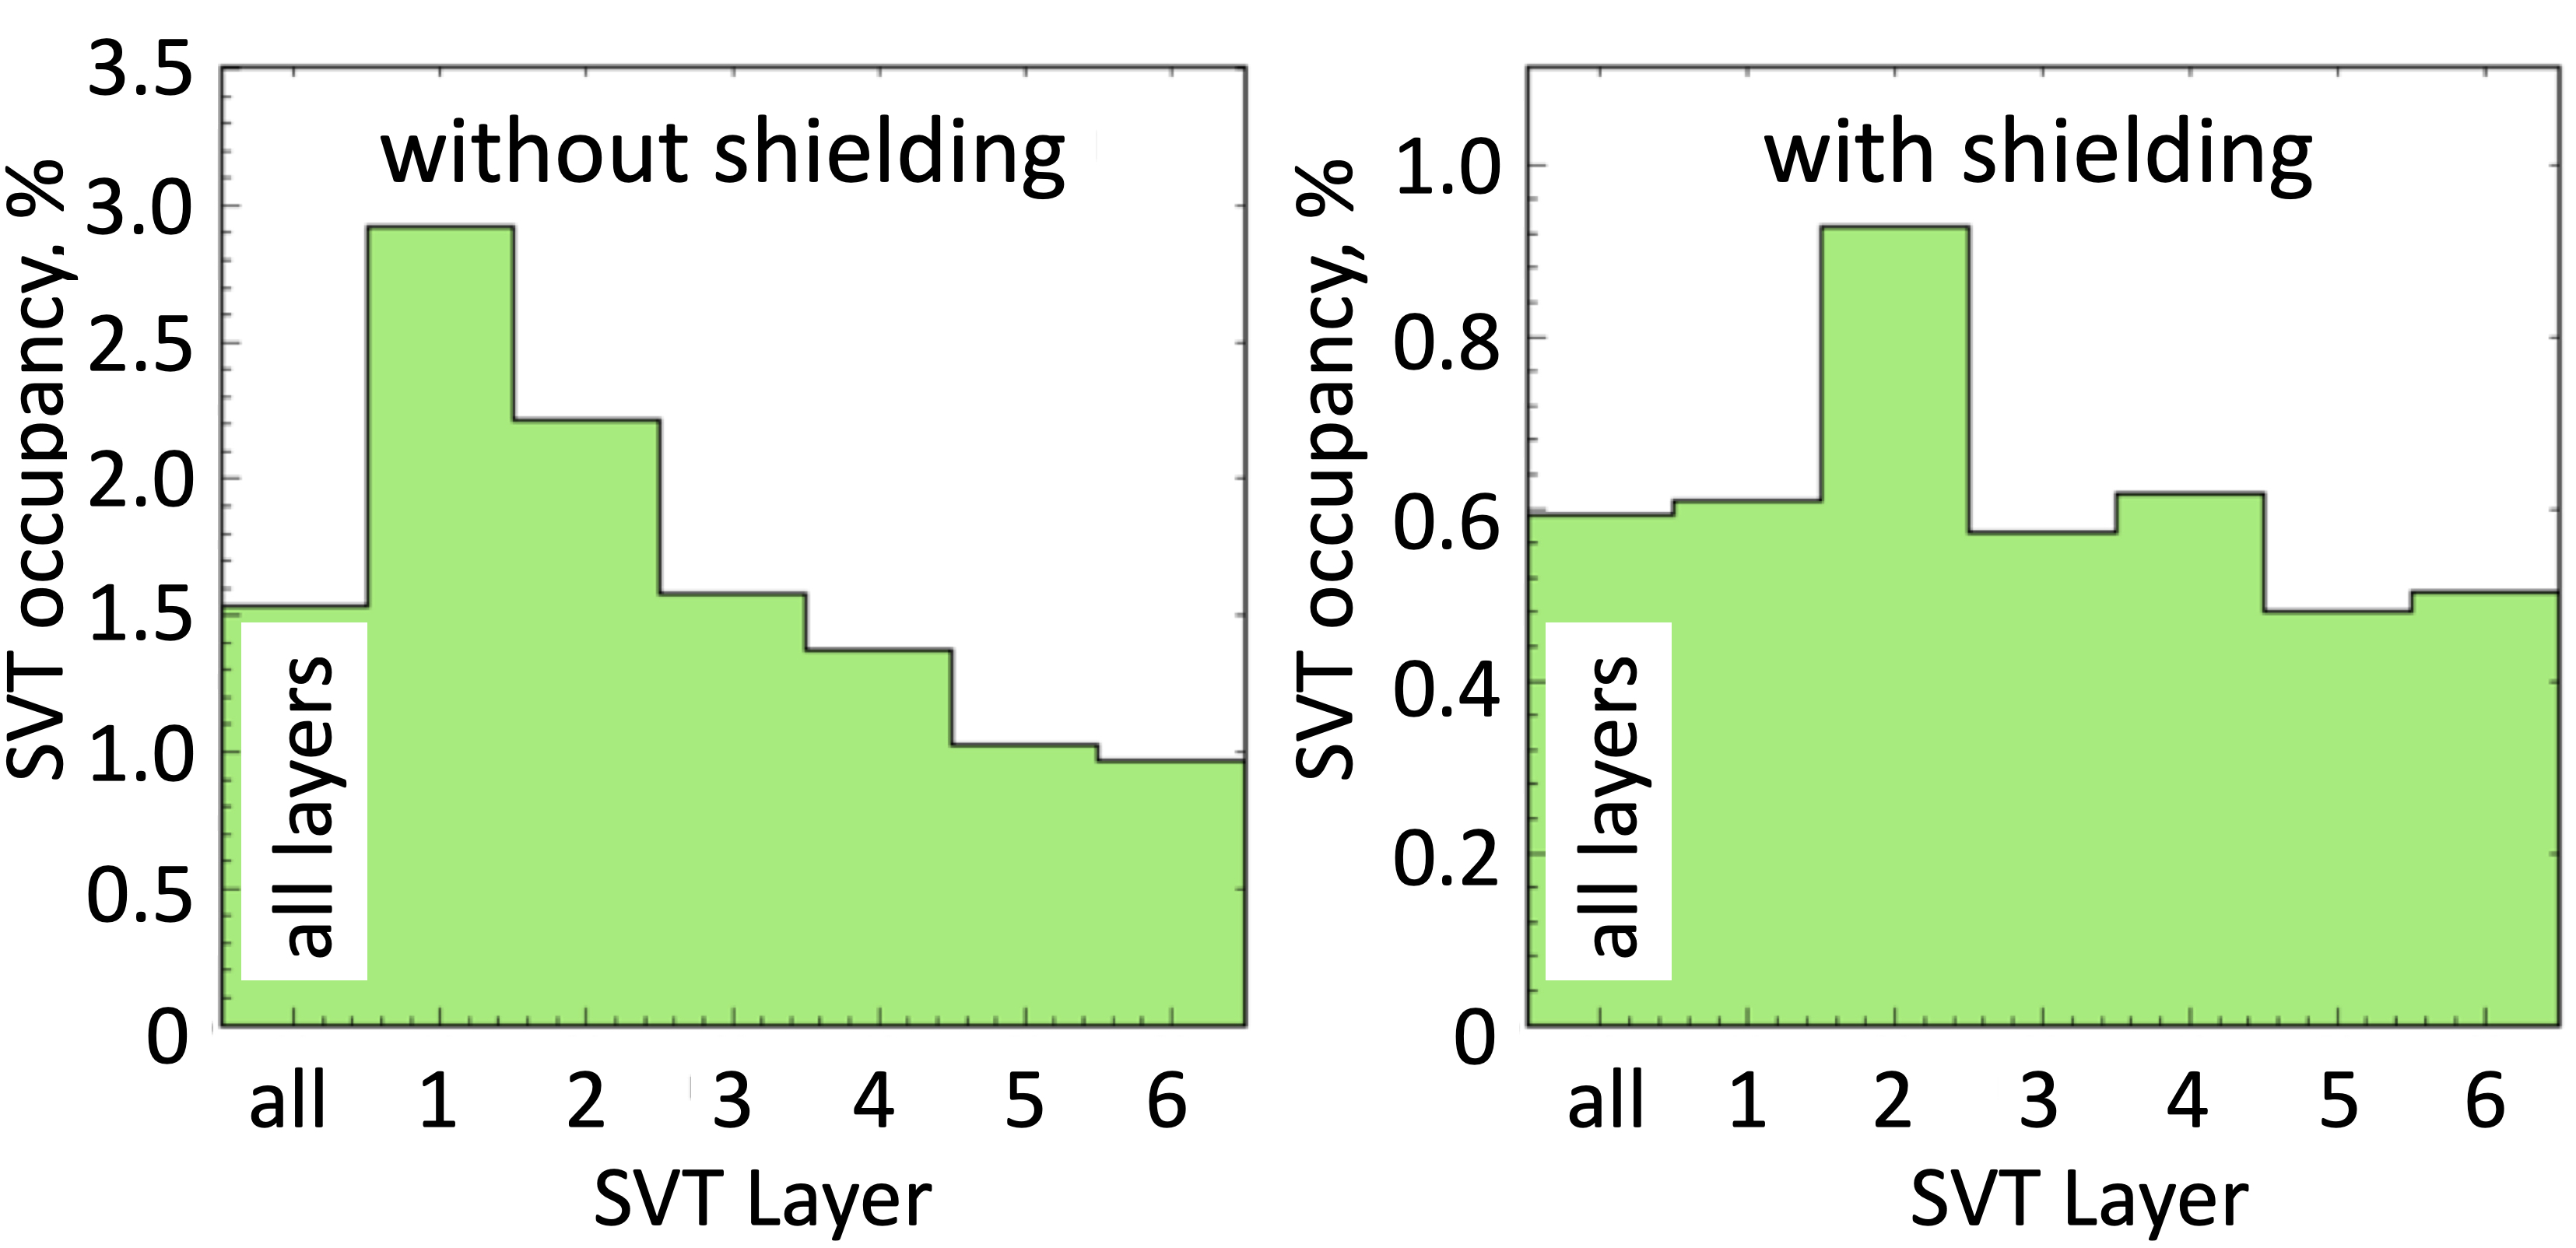
\includegraphics[width=1.0\columnwidth,keepaspectratio]{hit-occupancy-shielding.jpg}
\caption{Hit occupancies with and without the 50~$\mu$m-thick tungsten shield installed outside of the target scattering chamber.}
\label{fig:hit-occupancy-shielding}
\end{figure}

The impact of the tungsten shield on the SVT occupancy is shown in Fig.~\ref{fig:hit-occupancy-shielding}. Occupancies in all SVT layers are substantially lower, which results in better tracking performance due to reduced combinatorics. The effect of the shield on momentum resolution is negligible~\cite{SHIELDNOTE}. For the liquid hydrogen target the occupancy in the innermost layer of the SVT is approximately 1$\%$, decreasing to 0.5$\%$ in the outermost layer. There is no hit efficiency loss due to the dead time of the readout system at such occupancies.

\begin{figure}[hbt] 
\centering 
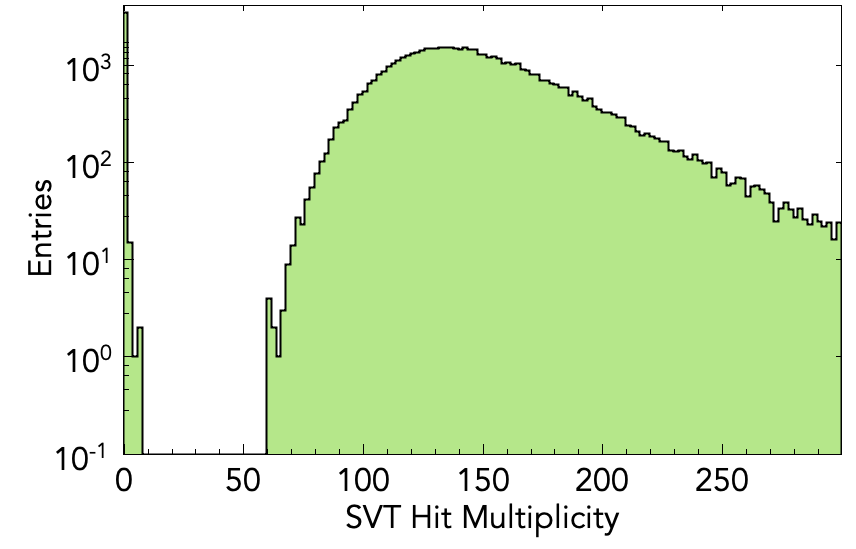
\includegraphics[width=1.0\columnwidth,keepaspectratio]{beam-no-beam-occupancy.png}
\caption{SVT hit multiplicity during the liquid hydrogen run at 50 nA beam current.}
\label{fig:beam-no-beam-occupancy}
\end{figure}

Noise performance of the SVT during the physics data taking is demonstrated in Fig.~\ref{fig:beam-no-beam-occupancy}, showing the SVT hit multiplicity during the liquid hydrogen run at nominal 50 nA beam current. The main peak is at about 130 hits per event which corresponds to 0.6$\%$ detector occupancy. The narrow peak on the left side represents SVT occupancy when there was no beam in the hall. The plot confirms good signal-to-noise ratio of the detector. 

\begin{figure}[hbt] 
\centering 
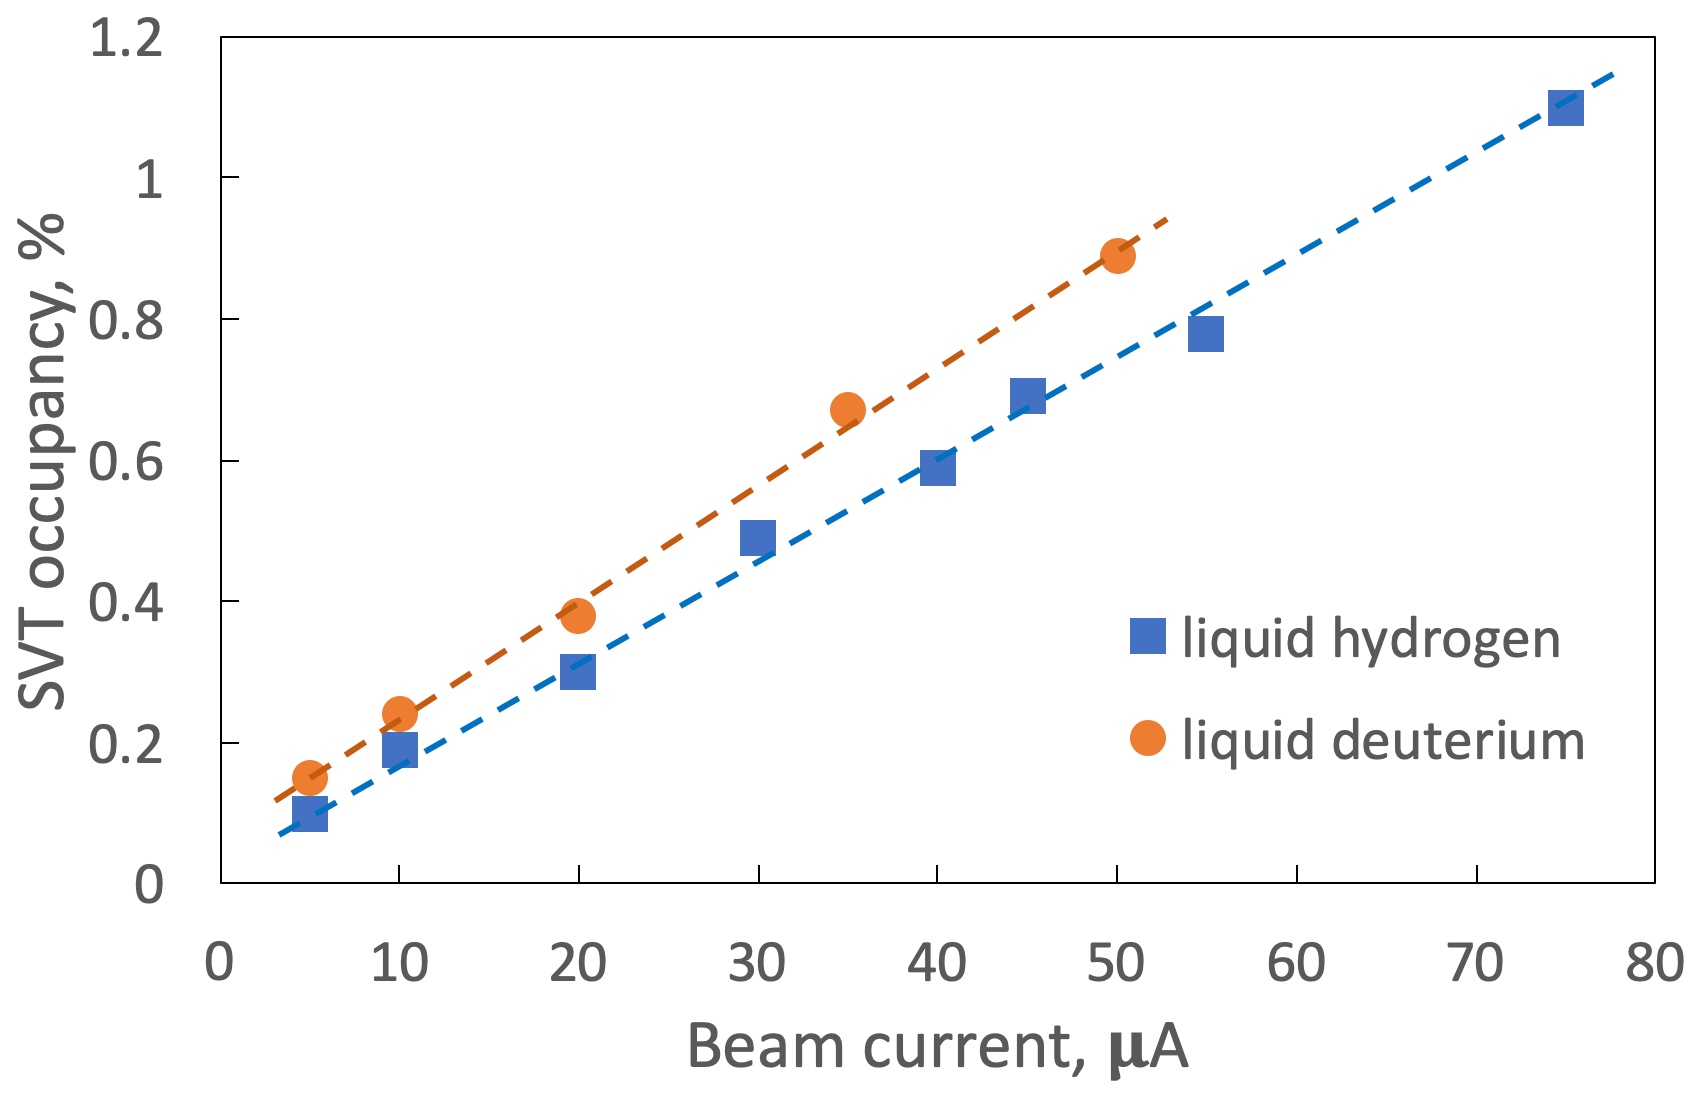
\includegraphics[width=1.0\columnwidth,keepaspectratio]{occupancy-beam-current.jpg}
\caption{SVT occupancy vs. beam current for hydrogen and deuterium targets.}
\label{fig:occupancy-beam-current}
\end{figure}

Fig.~\ref{fig:occupancy-beam-current} shows SVT occupancy vs. beam current for hydrogen and deuterium targets. The production data were taken at 50 nA. The SVT occupancy increases linearly with luminosity and remains at low levels not causing a substantial drop in the track finding efficiency.

\begin{figure}[hbt] 
\centering 
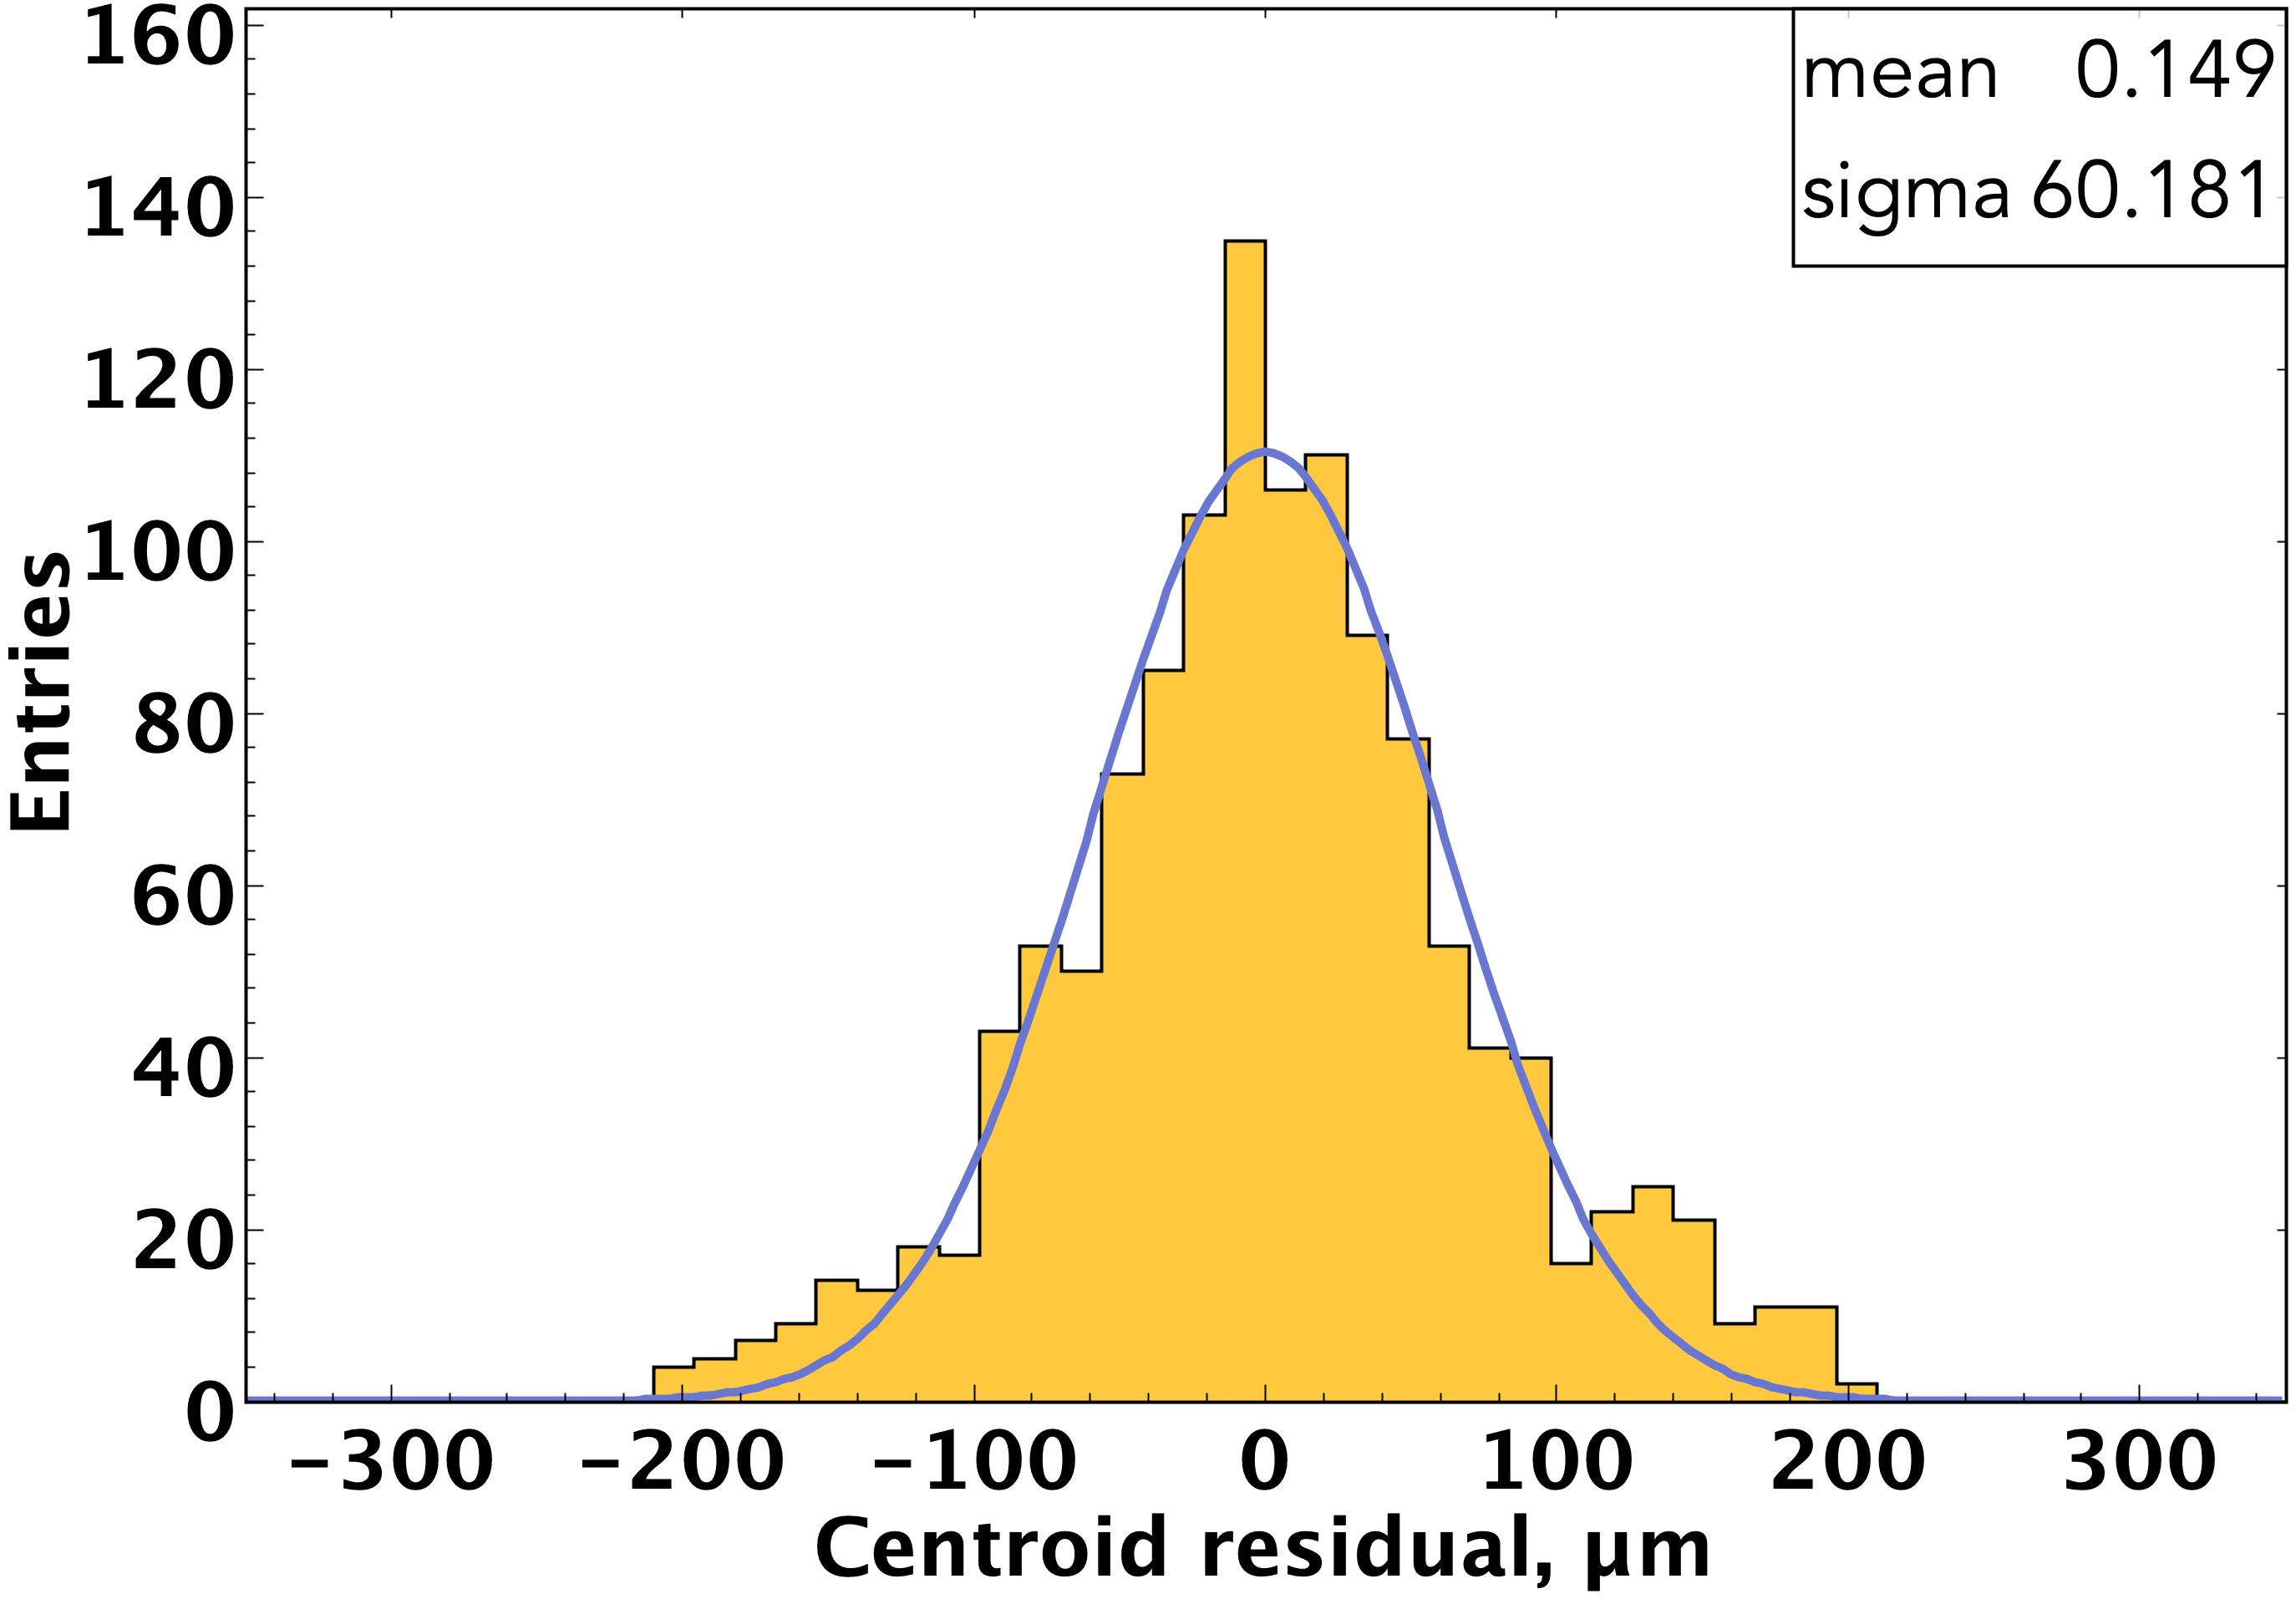
\includegraphics[width=1.0\columnwidth,keepaspectratio]{residual.jpg}
\caption{Centroid residual for one of the SVT sensors after preliminary tracker alignment.}
\label{fig:residual}
\end{figure}

A series of dedicated central tracker alignment runs was done at low beam current without magnetic field. The alignment data were collected when position of the central detector subsystems or the target has changed. The dependence of the residuals on the track parameters is explicitly taken into account. The alignment code uses the partial derivatives of the distance of closest approach (DOCA) taken with respect to the track parameters and the SVT geometry. This approach accounts for the correlated shifts among the geometry parameters. In addition to the track-based alignment, the data from the mechanical survey of the fiducials were also recorded when the detectors were moved. Centroid residual for one of the SVT sensors after preliminary tracker alignment is shown in Fig.~\ref{fig:residual}. Sensor spacial resolution is within the specs. Further improvements are expected from the ongoing development of the alignment algorithm and the track reconstruction code (like energy loss and Lorentz angle corrections which have strong impact on alignment).

\begin{figure}[hbt] 
\centering 
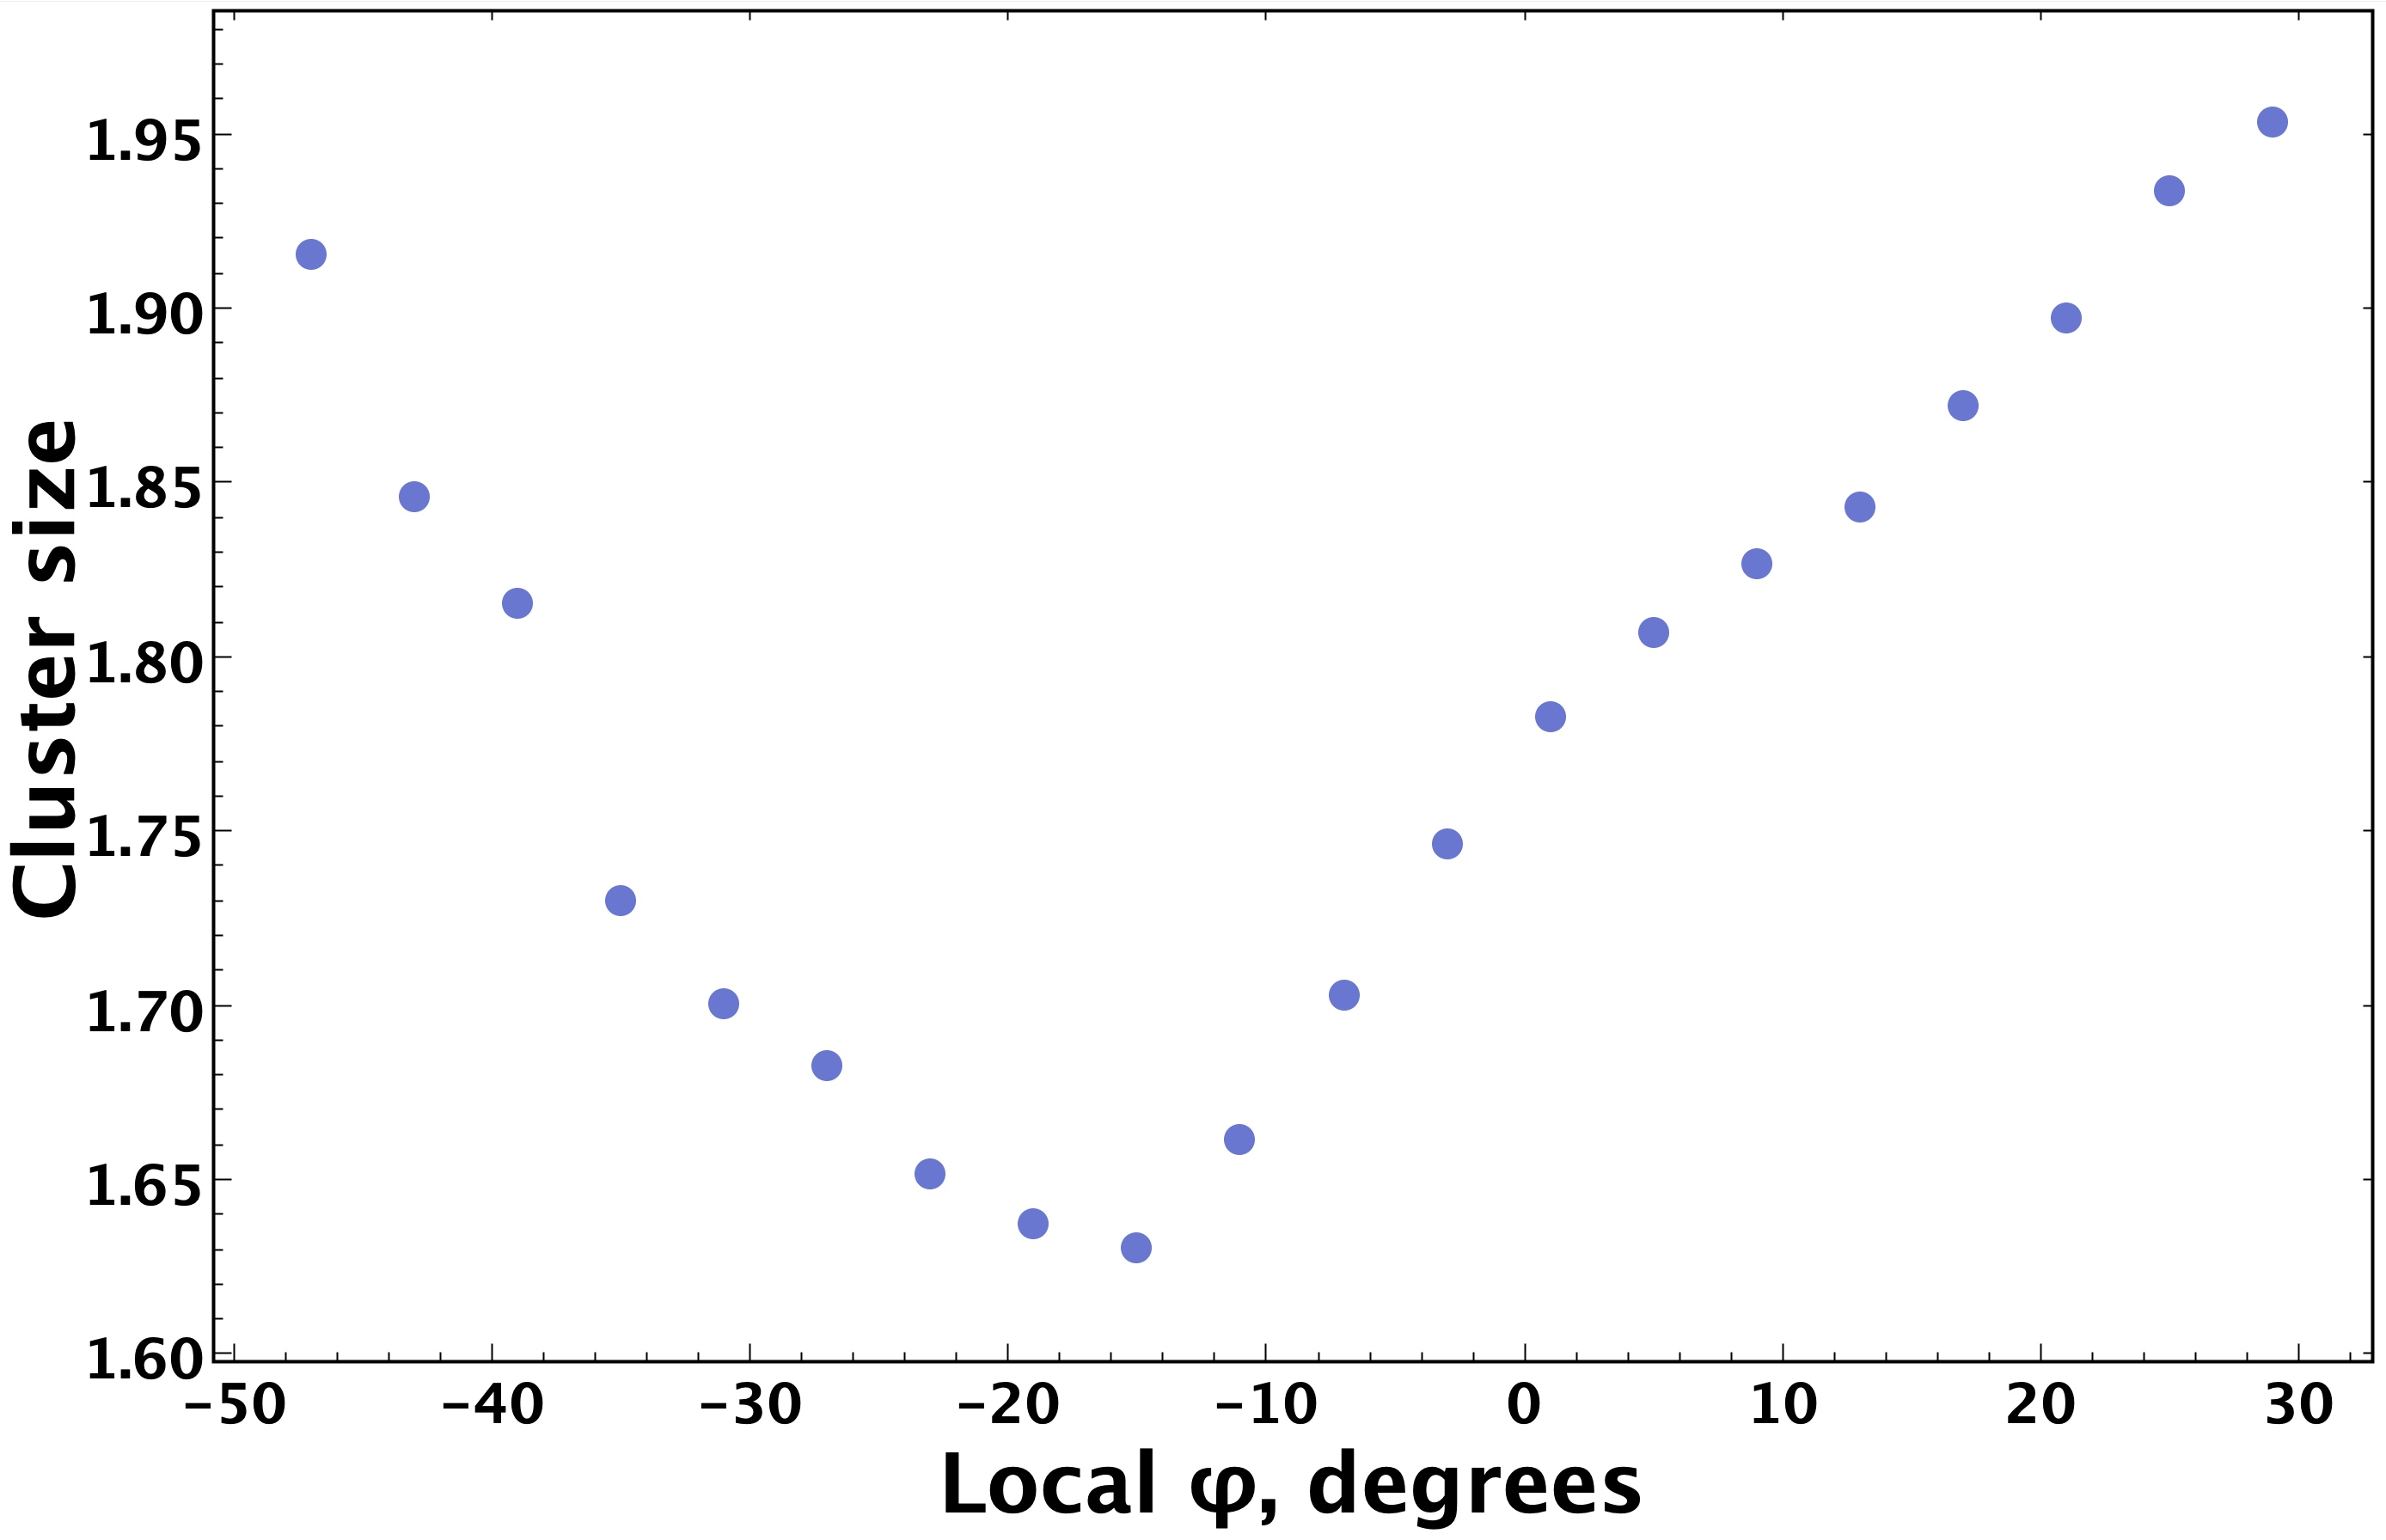
\includegraphics[width=1.0\columnwidth,keepaspectratio]{lorentz-angle.jpg}
\caption{Cluster size vs. local track azimuthal angle. The insert shows dependence of the cluster size on the track angle.}
\label{fig:lorentz-angle}
\end{figure}

In a strong magnetic field, charge in the silicon detector drifts at the Lorentz Angle, which must be taken into account when reconstructing the cluster position. Fig.~\ref{fig:lorentz-angle} shows average cluster size at different local azimuthal angles of the track. Zero angle is related to the normal incident tracks. The data were taken at negative polarity of the solenoid field. The Lorentz angle $\Theta_{LA}$ can be calculated as the track incidence angle corresponding to the minimum of the average cluster size when the track local angle is equal to the Lorentz angle.

\begin{figure}[hbt] 
\centering 
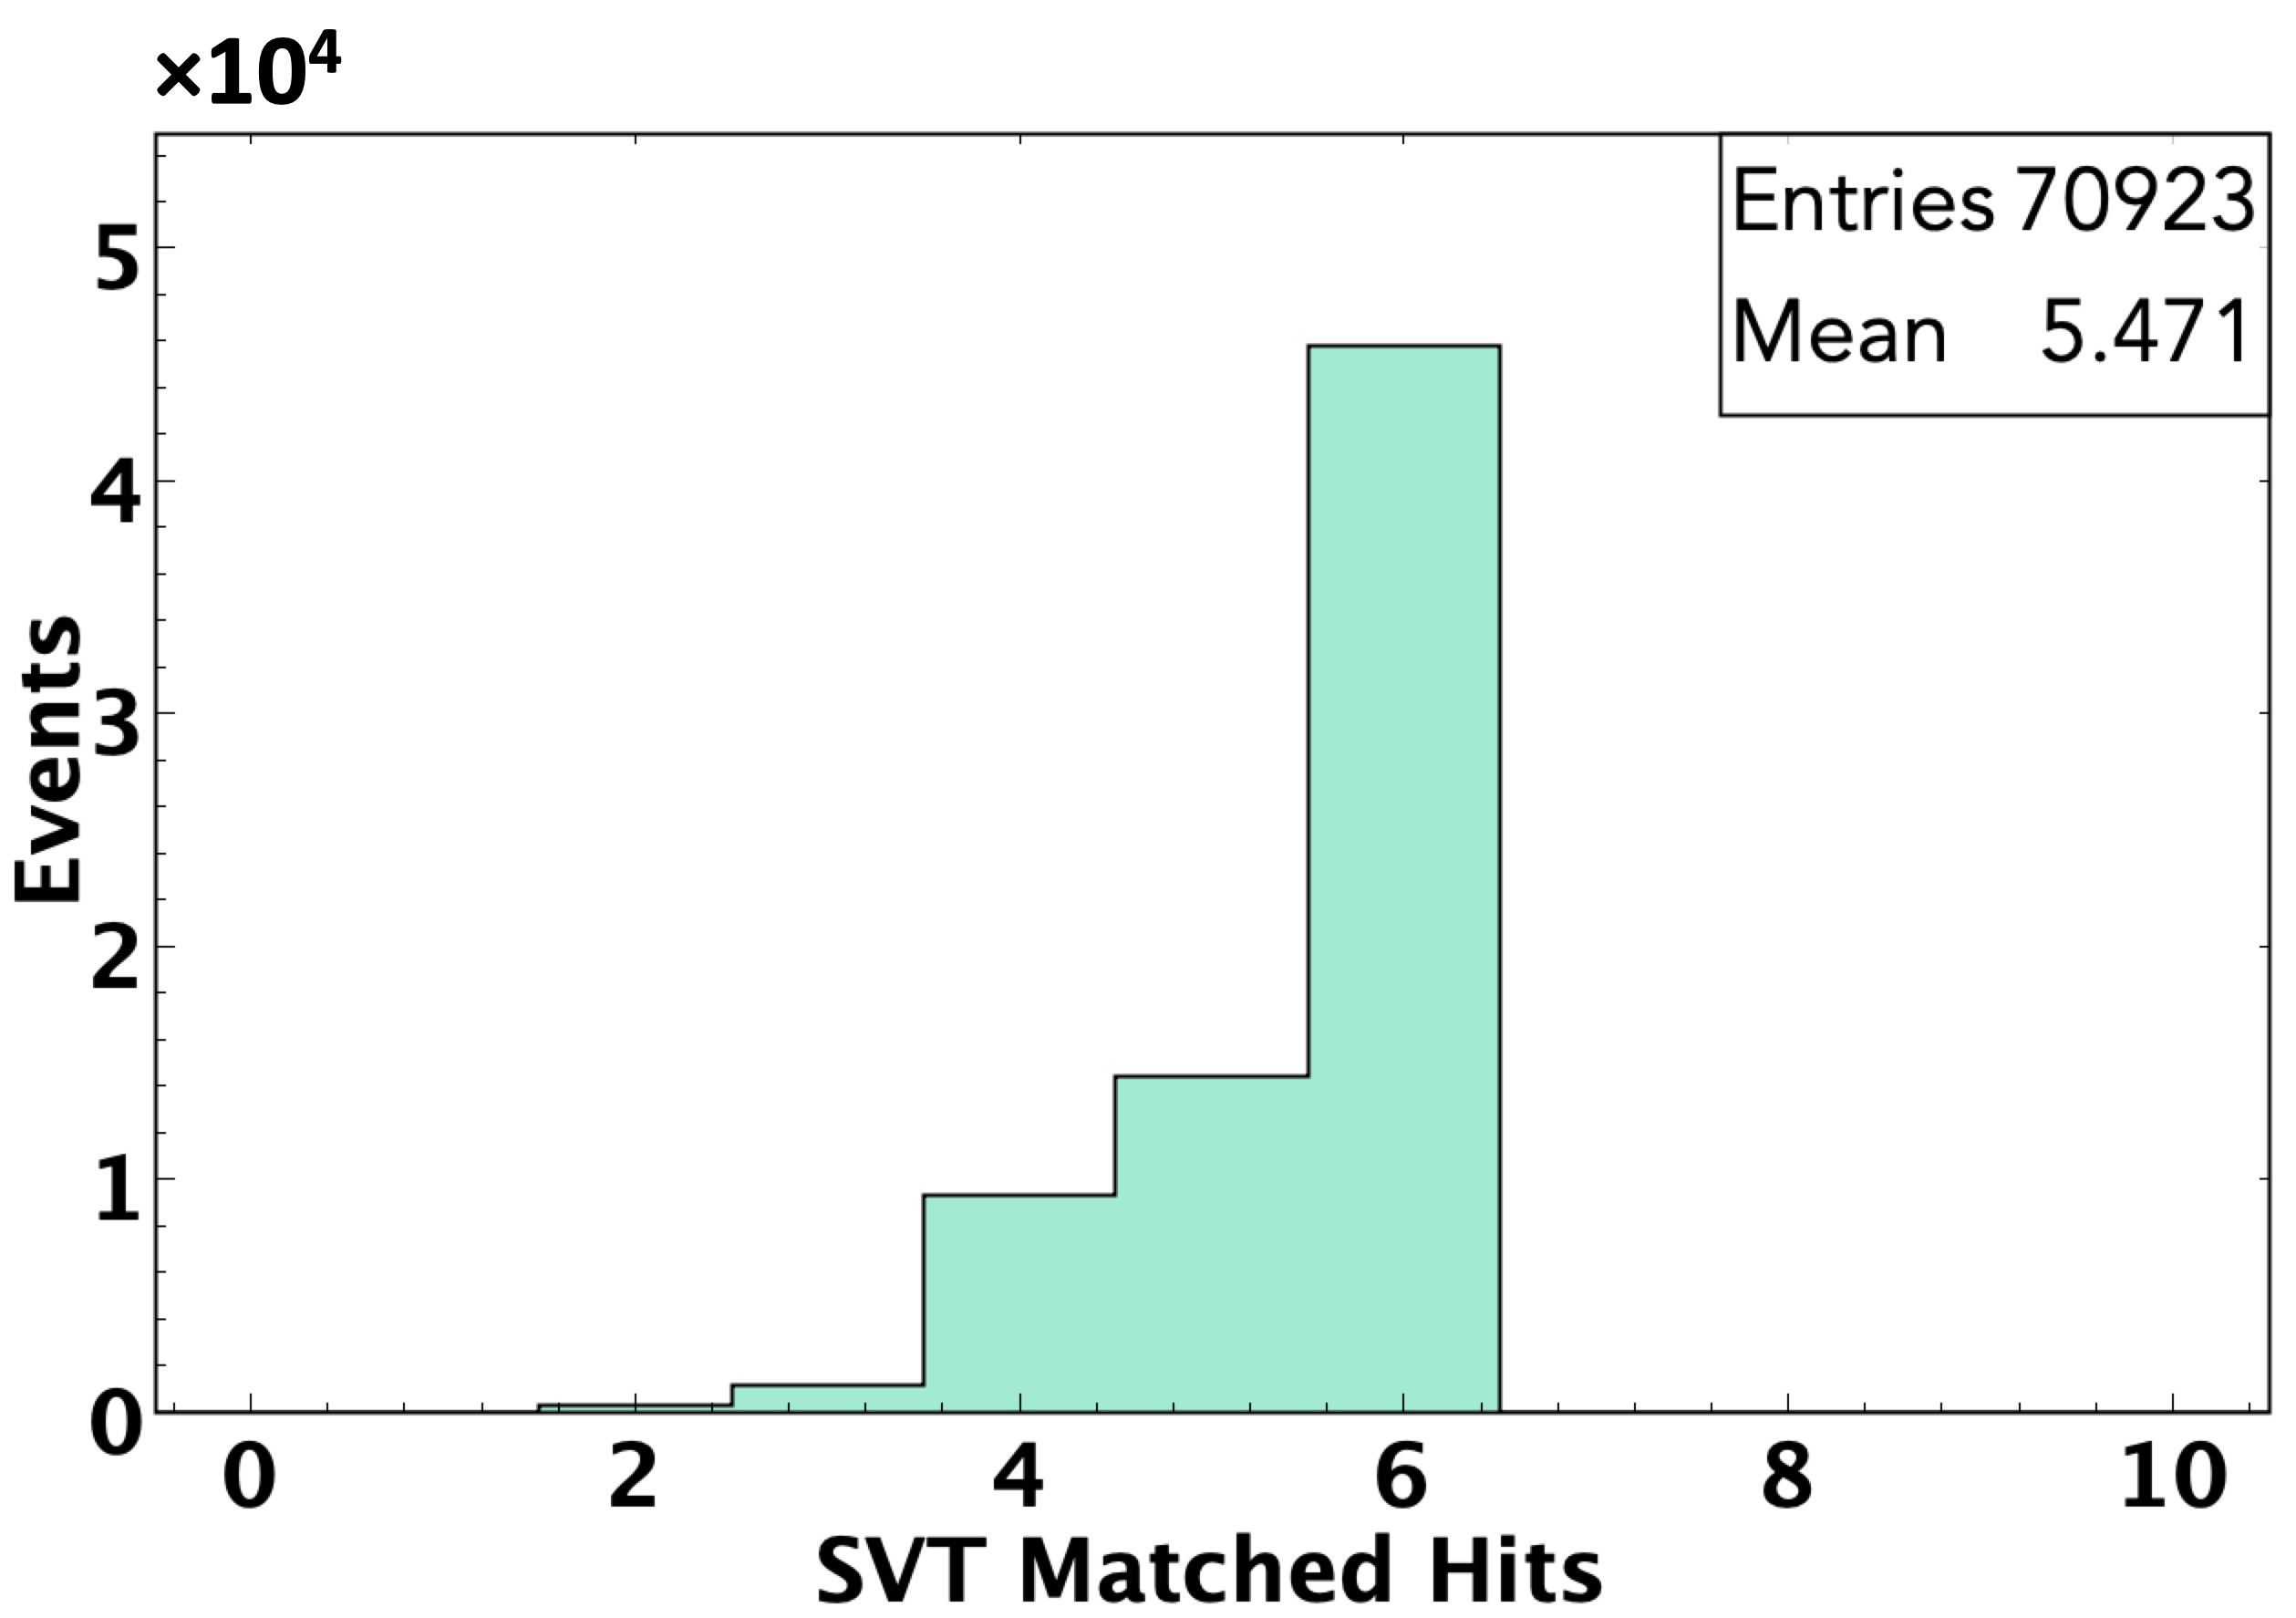
\includegraphics[width=1.0\columnwidth,keepaspectratio]{matched-hits.jpg}
\caption{Number of the SVT hits per track.}
\label{fig:matched-hits}
\end{figure}

The number of matched SVT hits per reconstructed track in the physics run with the hydrogen target is shown in Fig.~\ref{fig:matched-hits}. For most tracks all 6 SVT layers have been matched. The tracks with low number of matched hits passed through the gaps between the modules.


\begin{figure}[hbt] 
\centering 
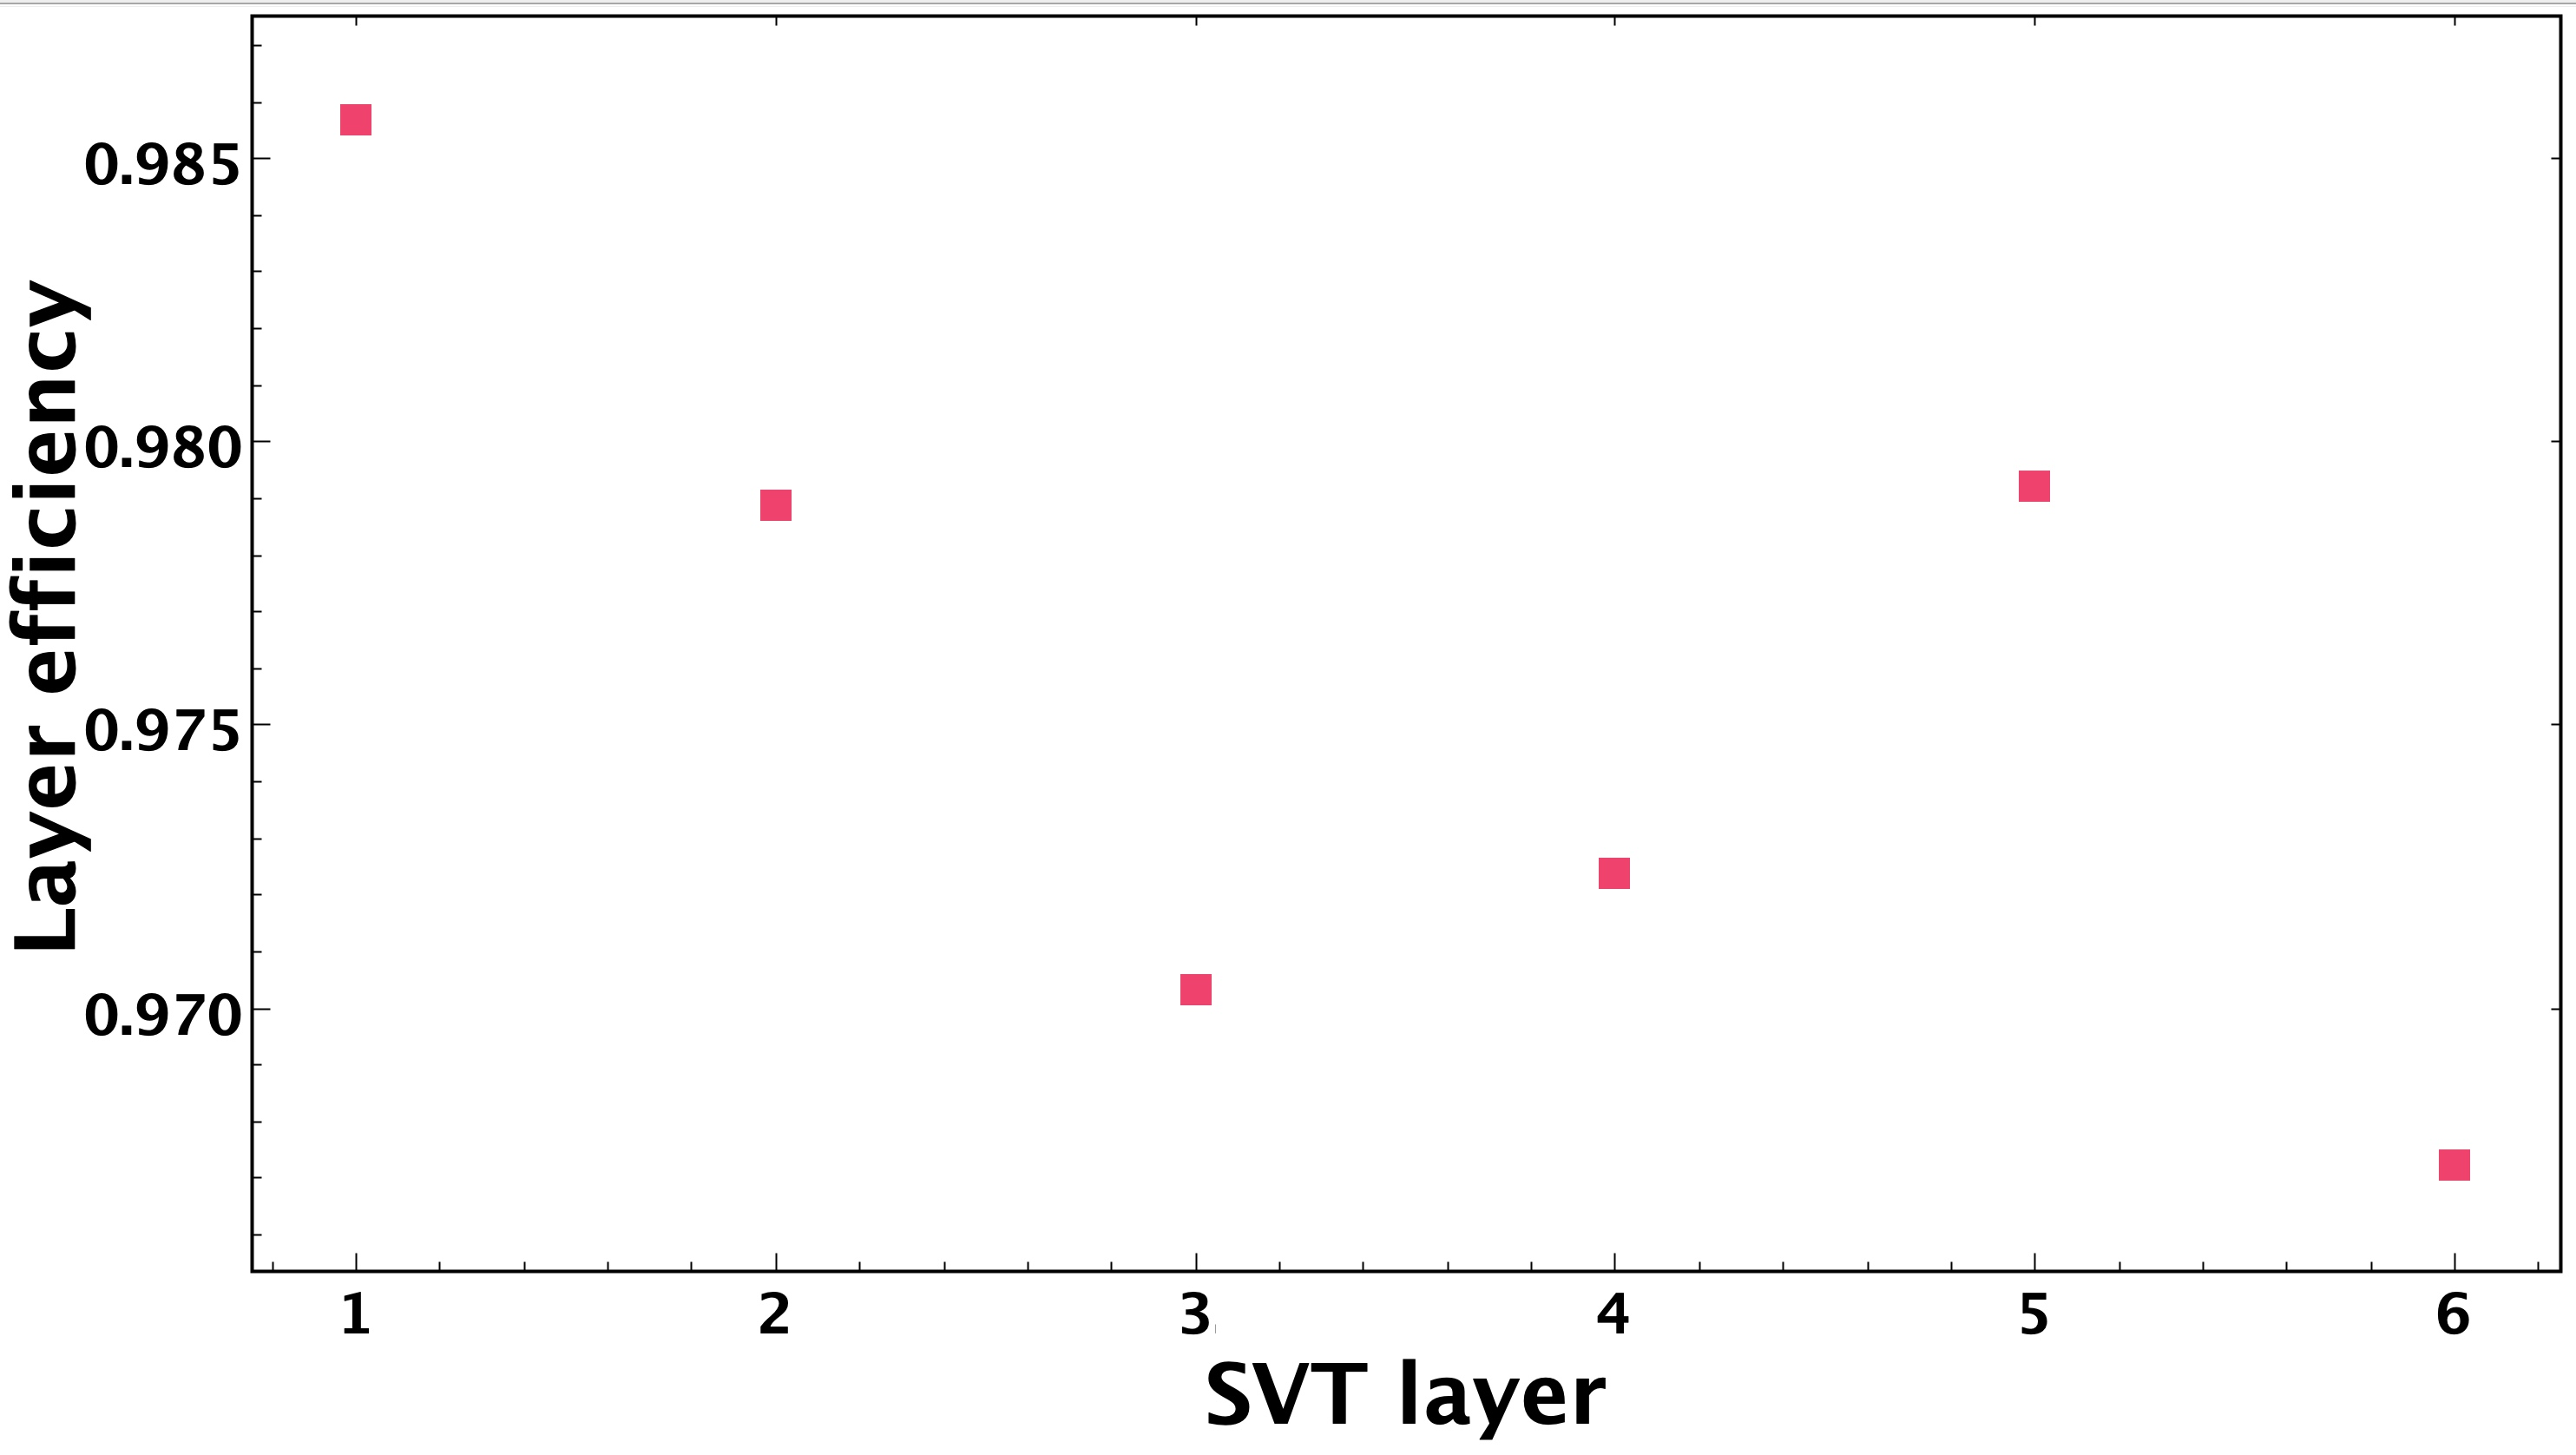
\includegraphics[width=1.0\columnwidth,keepaspectratio]{layer-efficiency.jpg}
\caption{Efficiency of hit matching in the SVT layers.}
\label{fig:layer-efficiency}
\end{figure}

Fig.~\ref{fig:layer-efficiency} shows efficiency of matching the hits to the tracks in each SVT layer. The hit is matched if it is associated with a track and there are on-track hits in two adjacent layers. The lower efficiency in the outer SVT layer is due to the tracks which are not within its acceptance. The efficiencies are expected to improve with further development of the tracking and alignment algorithms. 
